\documentclass[a4paper,11pt]{article}
\usepackage{amsmath, amssymb, amsthm, amsfonts, mathtools}
\usepackage[utf8]{inputenc}
\usepackage[T1]{fontenc}
\usepackage{comment}
\usepackage{marginnote}
\usepackage{booktabs}
\usepackage{tikz, tikz-cd}
\usepackage{hyperref}
\usepackage{geometry}
\usepackage[english, ngerman]{babel}
\usepackage{csquotes}
\usepackage[backend=biber, style=numeric, sorting=none]{biblatex}
\usepackage{BA_Titelseite}

%Namen des Verfassers der Arbeit
\author{Paul Jin Robaschik}
%Geburtsdatum des Verfassers
\geburtsdatum{25. Juni 2004}
%Gebortsort des Verfassers
\geburtsort{K\"oln}
%Datum der Abgabe der Arbeit
\date{\today}

%Name des Betreuers
% z.B.: Prof. Dr. Peter Koepke
\betreuer{Betreuer: Prof. Dr. Markus Hausmann}
%Name des Zweitgutachters
\zweitgutachter{Zweitgutachterin: Dr. Elizabeth Tatum}
%Name des Instituts an dem der Betreuer der Arbeit t�tig ist.
%z.B.: Mathematisches Institut
\institut{Mathematisches Institut}
%\institut{Institut f\"ur Angewandte Mathematik}
%\institut{Institut f\"ur Numerische Simulation}
%\institut{Forschungsinstitut f\"ur Diskrete Mathematik}
%Titel der Bachelorarbeit
\title{Bordism Homology and Cohomology}
%Do not change!
\ausarbeitungstyp{Bachelorarbeit Mathematik}


\newtheorem{definition}{Definition}[section]
\newtheorem{theorem}[definition]{Theorem}
\newtheorem*{remark}{Remark}
\newtheorem{proposition}[definition]{Proposition}
\newtheorem{lemma}[definition]{Lemma}
\newtheorem{corollary}[definition]{Corollary}
\newtheorem*{example}{Example}
\newtheorem*{nonex}{Non-example}


\newcommand{\demph}[1]{{\underline{{\textbf{#1}}}}}
\newcommand{\restrict}[1]{_{|_{#1}}}
\def\R{\mathbb{R}}

\addbibresource{sources.bib}

\begin{document}
\maketitle
\selectlanguage{english}
\tableofcontents\newpage

\begin{comment}
\newgeometry{
	left=20mm, % left margin
    top=25mm,
    right=20mm, % right margin
	%textwidth=150mm, % main text block
	%marginparsep=5mm, % gutter between main text block and margin notes
	%marginparwidth=40mm, % width of margin notes
  bmargin=2cm % height of foot note space
}
\end{comment}

\setcounter{section}{-1}

\addcontentsline{toc}{section}{Zusammenfassung}
\section*{\todo{Zusammenfassung}}
\todo{Hier eine deutsche Zusammenfassung der Arbeit}

\section{Introduction/Motivation}
%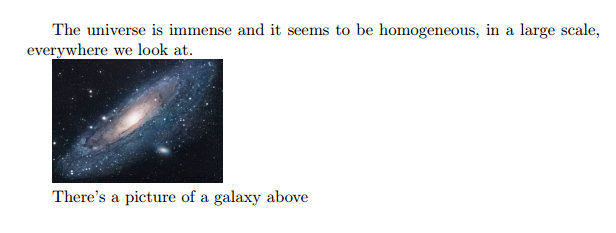
\includegraphics{galaxy.png}

Recall the definition of homotopy groups \(\pi_n(X)\) as the set of pointed homotopy classes of maps from the \(n\)-sphere \(S^n\) to a space \(X\). 
The problem with homotopy groups is that they are, in general, hard to compute, even for simple spaces such as spheres.\\
\todo{The general idea of bordism is to replace the \(n\)-sphere with a manifold of dimension \(n\) and to consider the homotopy classes of maps from this manifold to a space \(X\).}

\todo{more detail here}

%Testing citations:\cite{atiyah},\cite{brocker},\cite{thom},\cite{lee},\cite{hatcher},\cite{dieck},\cite{luck}

\section{Bordism}

\subsection{Manifolds}

\begin{definition}[Topological manifold\ {\cite[pp.2-3]{lee}}]
    An \(n\)-dimensional \demph{topological manifold} is a topological space \(M\) such that:
    \begin{itemize}
        \item \(M\) is Hausdorff, i.e.\ any two distinct points can be separated by disjoint open sets,
        \item \(M\) is second countable, i.e.\ there exists a countable basis for the topology of \(M\) and
        \item \(M\) is locally Euclidean i.e.\ every point in \(M\) has a neighbourhood homeomorphic to an open subspace of \(\mathbb{R}^n\).
    \end{itemize}
    We will often write \(M^n\) for an \(n\)-dimensional manifold.\ \(n\)-dimensional manifolds are also called \demph{\(n\)-manifolds}.
\end{definition}

\todo{maybe charts here}

\begin{example}
    \(\mathbb{R}^n\) is an \(n\)-dimensional topological manifold.
\end{example}

\begin{example}\label{sphere chart}
    The \(n\)-dimensional sphere \(S^n\) is an \(n\)-dimensional topological manifold. Hausdorffness and second countability follow from \(S^n\subset \mathbb{R}^{n+1}\). For local Euclideanness, we can use charts onto the open ball \(B_1^n(0)\)
     \[\varphi_i^\pm:U_i:=\{(x_0,\dots,x_n)\in S^n\mid \pm x_i>0\}\to B_1^n(0)\] by \[(x_0,\dots,x_i,\dots,x_n)\mapsto(x_0,\dots,x_{i-1},x_{i+1},\dots,x_n)\]
\end{example}

\begin{nonexs}
    %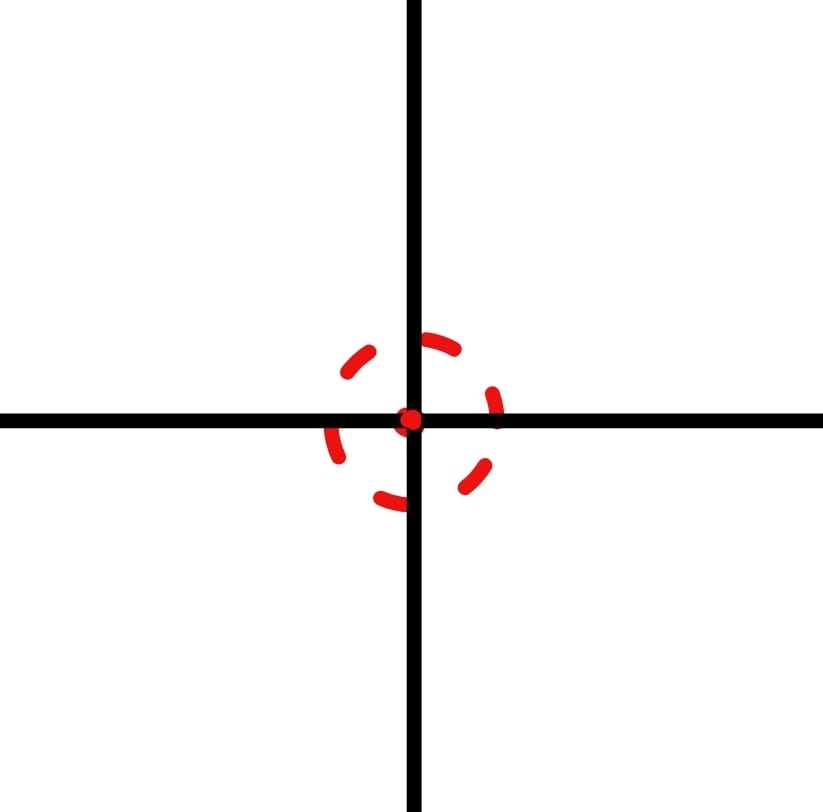
\includegraphics[width=0.2\textwidth]{cross}
    \begin{itemize}
        \item A \enquote{cross} in \(\mathbb{R}^2\) (\(\{(x_1,x_2\mid x_1=0 \lor x_2=0)\}\)) is not a topological manifold, because it is not locally Euclidean at the crossing point. 
        \item The line with two origins (\((\R\times\{0\}\dis\R\times\{1\})\big/((x,0)\sim(y,1)\Leftrightarrow (x=y \land x\neq 0))\)) is not a topological manifold. It is not Hausdorff, as the two origins cannot be separated by disjoint open sets. However, it is locally Euclidean.
        \item Let \(\{\pt\}\) denote the point space.\ \(\coprod_{i\in \mathbb{R}}\{\pt\}\) is not a topological manifold, because it is not second countable, as it has uncountably many connected components.
        \item \(S^1\dis\{\pt\}\) is not a topological manifold, because it is, locally homeomorphic to \(\mathbb{R}^1\) for any point in \(S^1\) or \(\mathbb{R}^0\), if the chosen point is not in \(S^1\), and the dimension of a manifold needs to be constant.
    \end{itemize}
\end{nonexs}

\begin{remark}
    One could replace the condition of being second countable with the condition of being paracompact (i.e.\ every open cover of \(M\) admits a locally finite refinement). The following equivalence holds for any topological space:
    \[\text{second countable}\iff \text{paracompact and countably many connected components}\]
    %This is shown in\ \cite{lee}. --- It is not :(
\end{remark}

%Being a topological manifold is just a property of a topological space \(M\). We will give manifolds extra structure by defining a smooth structure on them.

\begin{definition}[Chart]
    For a manifold \(M^n\), a \demph{chart} is a pair \(U,\varphi\) of an open subset \(U\subset M\) and a map \(\varphi:U\to\R^n\) such that \(\varphi:U\to\varphi(U)\) is a homeomorphism.
\end{definition}

\begin{definition}[(Smooth) Atlas\ {\cite[p.12]{lee}}]
    Let \(M\) be a topological manifold. A \demph{(smooth) atlas} \(\mathcal{A}\) on \(M\) is a collection of charts \((U_\alpha,\varphi_\alpha)\) such that:
    \begin{itemize}
        \item the \(\{U_\alpha\}\) cover \(M\),
        \item the charts are pairwise smoothly compatible, i.e.\ the transition functions 
        \(\varphi_j \circ \varphi_i^{-1}:\R^n\supset\varphi_i(U_i\cap U_j)\to\varphi_j(U_i\cap U_j)\subset\R^n\) are smooth.
    \end{itemize}
\end{definition}

\begin{example}
    The charts we chose for the \(n\)-sphere \(S^n\) in example\ \ref{sphere chart} form a smooth atlas on \(S^n\).
\end{example}

\begin{definition}[Equivalence of atlases]\label{equivalence atlas}
    Two atlases \(\mathcal{A}\) and \(\mathcal{A}^\prime\) (on a fixed topological manifold) are said to be \demph{equivalent}, if their union is still an atlas.
\end{definition}

%It can be shown that this is indeed an equivalence relation, but I will omit the proof here.

\begin{definition}[Smooth manifold\ {\cite[p.13]{lee}}]
    A \demph{smooth manifold} \(M=(M,[\mathcal{A}])\) consists of
    \begin{itemize}
        \item a topological manifold \(M\),
        \item an equivalence class \([\mathcal{A}]\) of smooth atlases on \(M\).
    \end{itemize}
\end{definition}

\begin{definition}[Smoothness of maps]
    A map \(f:(M^m,\mathcal{A})\to (N^n,\mathcal{B})\) between two smooth manifolds is said to be \demph{smooth}, if for all \(p\in M\), there exists a chart \((U,\varphi)\in\mathcal{A}\) such that \(p\in U\) and \((V,\psi)\in\mathcal{B}\) such that
    \begin{itemize}
        \item \(f(U\subset V)\)
        \item \(\psi\circ f\circ \varphi^{-1}:\varphi(U)\subset \R^m\to R^n\) is smooth as a map from \(\R^m\) to \(\R^n\).
    \end{itemize}
\end{definition}

\noindent\textit{Notation:}
    For two smooth manifolds \(M,N\), when writing \(M=N\), we will mean that they are diffeomorphic, i.e.\ there exists a bijective map \(f:M\to N\) such that \(f\) and \(f^{-1}\) are smooth. 
    %\todo{(We say a map \(f\) between two manifolds \(M^m,N^n\) is smooth, if for all \(p\in M\), there exist  charts \((U\ni p,\varphi)\) and \((V\subset N,\psi)\), such that 
    %(i) \(f(U)\subset V\) and 
    %(ii) \(\psi\circ f\circ \varphi:\varphi(U)\subset \R^m\to\R^n\) is smooth.)}


\begin{example}[Spheres]
    The \(n\)-sphere \(S^n\) with the atlas given by the charts in example\ \ref{sphere chart} is a smooth manifold.
\end{example}

\begin{example}[Subset of manifolds]
    For a smooth manifold \(M,[\mathcal{A}]\) any open subset \(U\) of \(M\) is a smooth manifold. 
    The atlas is given by restriction of the charts in \([\mathcal{A}]\) to \(U\). 
    We call \(U\) an \demph{open submanifold} of \(M\).
\end{example}

\begin{example}[Product of manifolds]
    For smooth manifolds \(M^m,N^n\), the product \(M\times N\) is a smooth \((m\cdot n)\)-manifold with the charts\[\{(U\times V,(\varphi,\psi))\mid(U,\varphi),(V,\psi)\text{ charts of }M,N\}\]
\end{example}

\begin{remark}
    While being a topological manifold is just a property of the topological space \(M\), being a smooth manifold gives the manifold extra structure.
\end{remark}

\begin{example}
    \((\mathbb{R},[(\mathbb{R},\mathrm{id})])\) and \((\mathbb{R},[\mathbb{R},x\mapsto x^3])\) are different smooth manifolds, because the transition functions between the charts are not smooth: 
    \(\mathrm{id}\circ{(x\mapsto x^3)}^{-1}=\varphi\), where
    \[\varphi(x)=\begin{cases}x^{\frac13} & x\geq0\\ -\lvert x\rvert^{\frac13}\end{cases}\]
    \(\varphi\) is not differentiable at 0, hence the atlases are not equivalent.\\
    However, they are diffeomorphic, as the map \(\varphi\) is a diffeomorphism between the two manifolds: 
    \((x\mapsto x^3)\circ \varphi\circ \id^{-1}= \id\). Its inverse is given by \(x\mapsto x^3\), which is also smooth: \(\id\circ (x\mapsto x^3)\circ{(x\mapsto x^3)}^{-1}=\id\)
\end{example}

%I am confused a bit, doesn't the diffeomorphism have to be smooth?? Check again.

\begin{example}[Exotic spheres]
    There exist 15 pairwise non-diffeomorphic smooth structures on \(S^7\). See\ \cite{kervaire} for a construction of these exotic spheres.
\end{example}

\begin{definition}[Manifold with boundary\ {\cite[p.25]{lee}}]
    To define a (smooth or topological) \demph{manifold with boundary}, replace the condition of the manifold being locally Euclidean with the condition that every point has a neighbourhood homeomorphic to an open subspace of the half space \(\mathbb{H}^n:=\{(x_1,\dots,x_n)\in\mathbb{R}\mid x_1\geq0\}\). Naturally, the charts now map into \(\H^n\) instead of \(\R^n\).
\end{definition}

\begin{comment}
\begin{definition}[Manifold]
    A \demph{smooth manifold with boundary} \(M=(M,[\mathcal{A}])\) is the data of a topological space \(M\) and an equivalence class \([\mathcal{A}]\) of smooth atlases such that:
    \begin{itemize}
        \item \(M\) is Hausdorff,
        \item \(M\) is second countable,
        \item \(\mathcal{A}\) is locally finite.
    \end{itemize}
\end{definition}
\end{comment}

\begin{remark}
    In this thesis, by \demph{manifold} we will always mean a smooth manifold with boundary, unless specified otherwise.
\end{remark}

\begin{definition}[Boundary\ {\cite[p.25]{lee}}]
    Let \(M^n\) be a manifold. A point \(x\in M^n\) is called an \demph{interior point} if it admits a neighbourhood homeomorphic to \(\mathbb{R}^n\). Otherwise, it is called a \demph{boundary point}.\\
    The set of interiour points is denoted by \(\mathrm{int}(M)\) and is called the \demph{interior} of \(M\). The set of boundary points is denoted by \(\partial M\) and is called the \demph{boundary} of \(M\).\\
    If \(M\) is compact and has empty boundary, \(M\) is called a \demph{closed manifold}. %If a manifold is compact and has non-empty boundary, it is called a \demph{compact manifold with boundary}. If a manifold is not compact, it is called an \demph{open manifold}
\end{definition}

\begin{example}
    \(([0,1],[([0,1],i)])\), where \(i\) is the inclusion into \(\mathbb{R}\), is a 1-manifold. Its boundary is \(\partial [0,1]=\{0,1\}\).
\end{example}

\begin{example}
    \(\mathbb{H}^n\) is a manifold with boundary \(\mathbb{R}^{n-1}\)
\end{example}

\begin{example}
    The \(n\)-disk \(D^n\) is a manifold with boundary \(S^{n-1}\)
\end{example}

\begin{theorem}[Boundaries are submanifolds]\label{boundary manifold}
    The boundary of an \(n\)-manifold is a closed \((n-1)\)-dimensional (embedded) submanifold.
\end{theorem}

\begin{proof}
    Let \((M^n,[\mathcal{A}])\) be a manifold. A smooth structure on \(\partial M\) is given by the restriction of the charts in \([\mathcal{A}]\) to \(\partial M\): \[\{(U\cap\partial M,\varphi\restrict{U\cap\partial M})\mid (U,\varphi)\in[\mathcal{A}]\}\]
    Smooth compatability follows from the smooth compatibility of the charts in \([\mathcal{A}]\). This makes \(\partial M\) a submanifold of \(M\). It remains to show that it is closed and of codimension \(1\). The charts in \([\mathcal{A}]\) map every point in \(\partial M\) to \(\partial\H^n=\R^{n-1}\). If they didn't, we could find a Euclidean neighbourhood of that point, contradicting the fact that it was a boundary point in \(M\). As the charts restricted to \(\partial M\) now map to \(\R^{n-1}\), we have an \((n-1)\)-dimensional submanifold without boundary.\\
    \unsure{Need: \(\varphi(U\cap\partial M)\) is open and \(\varphi(x)\notin\partial\H^n\) for \(x\) interior point}
\end{proof}

\begin{theorem}[Collar theorem \ {\cite[I, Satz 1.5]{brocker}}]\label{collar}
    Let \(M\) be a manifold. Then there exists a neighbourhood \(U\) of \(\partial M\) with a diffeomorphism \(s:\partial M\times [0,1)\to U\) with \(s(\partial M\times\{0\})=\partial M\). \(U\) is called a \demph{collar} of \(\partial M\) in \(M\).
\end{theorem}

\begin{proof}\todo{See\ \cite[p.223]{lee} for a proof. Maybe I want Br\"ocker, tom Dieck here}
\end{proof}

\begin{observation}
    If \(\partial M\) has multiple path components, then we can find a collar for each path component.
\end{observation}

\begin{theorem}[Smooth Urysohn lemma {\cite[Exercise 2-14]{lee}}]\label{urysohn}
    Let \(M\) be a manifold, \(A,B\subset M\) disjoint closed sets. Then, there is a smooth function \(f:M\to\R\) such that \(f\restrict{A}=0\) and \(f\restrict{B}=1\)
.
\end{theorem}

\begin{proof}
    \todo{this follows from the normality of manifolds and the existence of bump functions}
\end{proof}

\begin{definition}[Tangent space {\cite[p.72]{lee}}]
    The \demph{tangent space} of a manifold \(M^n\) at a point \(p\in M\), denoted by \(T_p M\) is the set of equivalence classes of smooth curves \(\gamma:[-\varepsilon,\varepsilon]\to M\), \(\gamma(0)=p\) under the equivalence relation \(\gamma_1\sim\gamma_2:\Leftrightarrow\) for any smooth function \(f:M\to\mathbb{R}^n\) defined in a neighbourhood of \(p\), we have \((f\circ\gamma_1)'(0)=(f\circ\gamma_2)'(0)\) (\(\varepsilon>0\) depends on \(\gamma\))
\end{definition}

\begin{remark}
    For an \(n\)-manifold, \(T_p M\) is an \(n\)-dimensional vector space over \(\R\) for every point \(p\in M\). \todo{reference}
\end{remark}

\begin{definition}[Differential {\cite[p.55]{lee}}]
    Let \(f:M\to N\) be a smooth map between two manifolds. For \(p\in M\), the \demph{differential of} \(f\) \demph{at} \(p\) is given by
    \[df_p:T_p M\to T_{f(p)}N\]
    \[[\gamma]\mapsto[f\circ \gamma]\]
\end{definition}

\begin{definition}[critical value {\cite[p.105]{lee}}]
    Let \(f:M\to N\) be a smooth map between two manifolds. A point \(p\in M\) is a \demph{critical point} of \(f\), if the differential \(df_p:T_p M\to T_{f(p)}N\) fails to be surjective. Otherwise, it is called a \demph{regular point}.\\
    A point \(q\in N\) is a \demph{critical value} of \(f\), if \(f^{-1}(q)\) contains a critical point of \(f\). Otherwise, it is called a \demph{regular value}.
\end{definition}

\begin{remark}
    For a smooth map \(f:M^n\to \R\), \(r\) a regular value of \(f\), \(\{p\in M:f(p)\leq r\}=f^{-1}(-\infty,r]\) is an \(n\)-dimensional submanifold of \(M\).\ \(f^{-1}(r)\) is an \((n-1)\)-dimensional submanifold of \(M\).\ \todo{reference}
\end{remark}

\todo{with a bit of measure theory, we can state this}

\begin{theorem}[Sard's theorem\ {\cite[Theorem 6.10]{lee}}]\label{sard}
    For a smooth map \(f:M\to N\) between two manifolds, the set of critical values of \(f\) has measure zero in \(N\).
\end{theorem}

\begin{proof}
    See\ \cite{lee} for a proof.
\end{proof}

\begin{definition}[Connected sum {\cite[Example 9.31]{lee}}]
    For two connected manifolds \(M^n,N^n\), choose smooth embeddings \(D^n\xhookrightarrow{i}\mathrm{int}(M)\), \(D^n\xhookrightarrow{j}\mathrm{int}(N)\). Then the connected sum of \(M\) and \(N\) is defined as \todo{could be done as pushout}
    \[M\#N:=((M\setminus i(\overset{\circ}{D^n}))\dis(N\setminus j(\overset{\circ}{D^n})))\big/(i(x)\sim j(x))\]
    for all \(x\in\partial D^n\).
    \begin{center}
        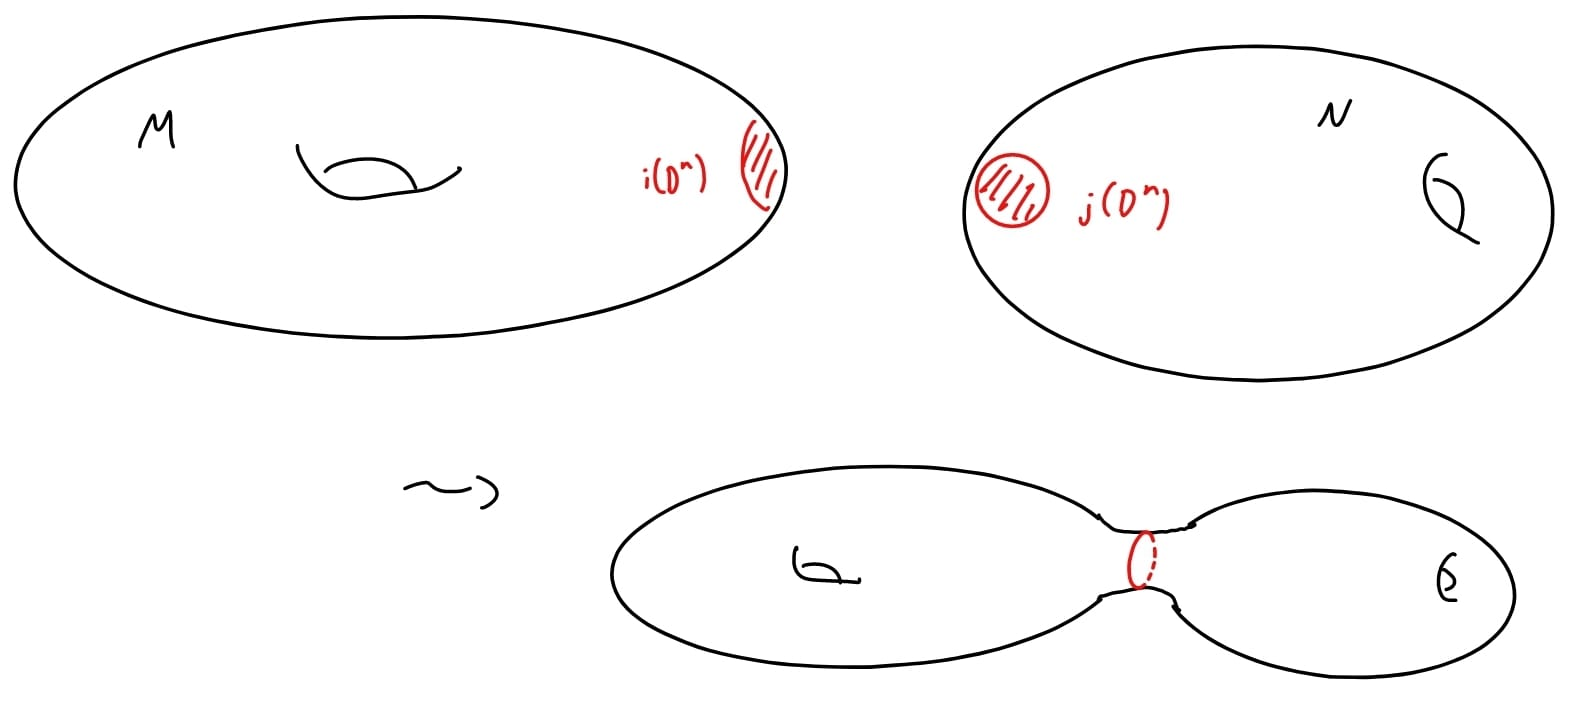
\includegraphics[width=0.6\textwidth]{connectedsum.jpg}
    \end{center}
\end{definition}

\begin{remark}
    This construction is a priori only unique up to homeomorphism. It can be shown that \(M\#N\) is a smooth manifold if \(M\) and \(N\) are smooth and that it is unique up to diffeomorphism, see\ \cite[VI, Theorem 1.1.]{kosinski} for \unsure{details}.
\end{remark}

%\begin{definition}[Separating function]
%    to be done. I need this in an example that still needs to be done (pair of pants).
%\end{definition}
%We can use this without calling it separating function.

%\section{Bordism}

One of the problems with working with manifolds is that they are, in higher dimensions, hard to classify up to homeomorphism or diffeomorphism. Bordism is a way to classify manifolds up to a weaker equivalence relation, which is \todo{easier to work with}. \todo{maybe in introduction}

\subsection{Unoriented Bordism}
\subsubsection{Definitions}
%Examples need to be added here, too.

\begin{definition}[Singular manifold\ {\cite[II, Definition 1.1]{brocker}}]\label{singular manifold}
    Let \(X\) be a topological space. An \(n\)-dimensional \demph{singular manifold} in \(X\) is a pair \((M,f)\) of a compact manifold \(M\) and a continuous map \(f:M\to X\).\\
    The \demph{boundary} of a singular manifold is \(\partial(M,f):=(\partial M, \partial f):=(\partial M,f\restrict{\partial M})\).
\end{definition}

\begin{definition}[Nullbordant\ {\cite[II, Definition 1.2]{brocker}}]
    Let \((M,f)\) be a singular \(n\)-manifold in \(X\). We say that \((M,f)\) is \demph{nullbordant}, if there exists a singular (\(n+1\))-manifold \((B,F)\) in \(X\), such that \(\partial(B,F)=(M,f)\).\\
    \(B,F\) is then called a \demph{nullbordism} of \((M,f)\).
\end{definition}

In the following, we will sometimes omit \(f\) from the notation, if it is clear, what \(f\) is, e.g.\ if \(X=\pt\) or \(M=\emptyset\)

\begin{example}
    For \(X=\pt\), and \(M=S^n\), we have a nullbordism \(B=D^{n+1}\), the disk.%\ (\(f\) can be omitted, as it is constant.)
\end{example}

\begin{example}
    For \(X=\pt\), and \(M=\T^2\), the torus, a nullbordism is \(S^1\times D^2\), the filled torus.
\end{example}

\begin{remark}
    These examples can be generalized to \(f\) just being a constant %maybe even nullhomotopic
    map, and \(B\) any manifold such that \(\partial B=M\). 
\end{remark}

\begin{example}
    For \(M=\emptyset\), any closed manifold is a nullbordism of \(M\), no matter what the space \(X\) is.% (Again, \(f\) can be omitted, as it is the empty map.)
\end{example}

\begin{observation}
    A singular manifold \((M,f)\) can be nullbordant even if \(f\) is not nullhomotopic.
\end{observation}

\begin{example}
    \(X=S^1\), \(M=S^1\), and \(f\) is given by wrapping around the circle twice, a nullbordism is given by the M\"obius strip \(\mathbb{M}\) with \(F\) as projection onto the circle.\begin{center} 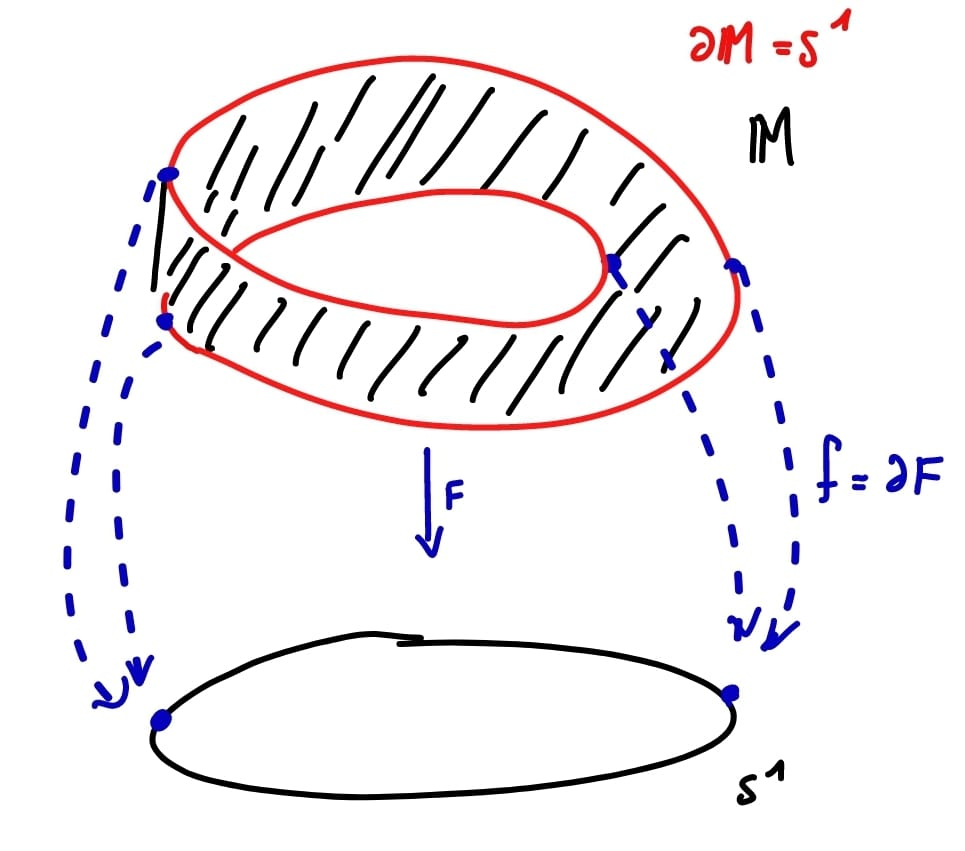
\includegraphics[width=0.4\textwidth]{mobius.jpg} \end{center}
\end{example}


\begin{definition}[Bordant\ {\cite[II, Definition 1.3]{brocker}}]\label{bordant}
    Let \((M,f)\) and \((N,g)\) be singular manifolds in \(X\). We say that \((M,f)\) and \((N,g)\) are \demph{bordant}, if their sum \((M,f)+(N,g):=(M+N, (f,g)):=(M\dis N, f\dis g)\) is nullbordant.

    A nullbordism of \((M,f)+(N,g)\) is called a \demph{bordism} between \((M,f)\) and \((N,g)\).
\end{definition}

We will refer to this relation as \demph{bordism relation}.

\begin{remark}
    \[(M,f)+(\emptyset,g) \text{ are bordant} \iff (M,f) \text{ is nullbordant}\]
\end{remark}

\begin{remark}
    It follows that \((M,f)\) and \((N,g)\) can only be nullbordant if \(M\) and \(N\) are of the same dimension.
\end{remark}

\begin{example}[Cylinder]\label{cylinder bordism}
    For an arbitrary \(X\), and \((M,f)=(N,g)\), we always get the cylinder as a bordism: \((M\times[0,1],f\circ\mathrm{pr}_1)\), where \(\mathrm{pr}_1\) is the projection onto the first factor.
    \begin{center}
        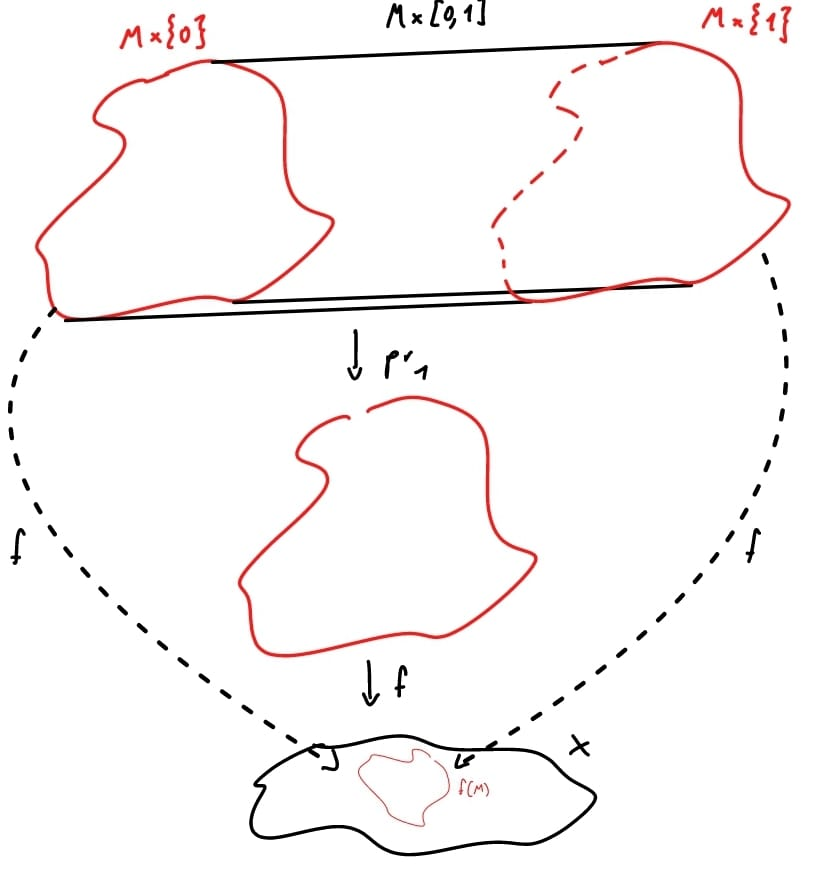
\includegraphics[width=0.4\textwidth]{cylinder.jpg}
    \end{center}
\end{example}
%Draw a picture

\begin{example}[Pair of pants]\label{pants}
    For \(X=\mathrm{pt}\), \(M_1=M^n\dis N^n\) and \(M_2=M\# N\), we get the \enquote{pair of pants} as a bordism between them. We can construct the pants as follows. Take the two cylinders \(M\times [0,1]\) and \(N\times[0,1]\). Now \[f:(M\times[0,1])\dis(N\times[0,1])\to [0,1]\]
    given by
    \[(p,t)\mapsto t\] regardless of \(p\in M\) or \(p\in N\) is a smooth map between manifolds. By theorem\ \ref{sard}, we may assume that \(\frac12\) is a regular value. We embed \(D^{n+1}\) by \(i\) and \(j\) into the cylinders such that \(f\circ i(0)=f\circ j(0)=\frac12\) and \(f\circ i(x)=f\circ j(x)\) for all \(x\in D^{n+1}\). 
    We may also assume that \({(f\circ i)}^{-1}(\frac{1}{2})\) and is connected, else we can just consider smaller disks inside the disks. 
    Taking the connected sum now with respect to \(i\) and \(j\) leaves 
    \[\tilde f:(M\times[0,1])\#(N\times[0,1])\to[0,1],\]
    which is induced  by \(f\), well-defined. Furthermore, \(\frac12\) is still a regular value of \(\tilde f\). 
    Note that \(\tilde{f}^{-1}=M\#N\), as the embeddings \(i,j\) induce embeddings of \(D^n\) into \(M,N\). 
    Now we define the pair of pants to be \(\tilde{f}^{-1}([0,\frac12])\), which is an \((n+1)\)-dimensional manifold by with boundary \(\tilde f^{-1}(0)\dis\tilde f^{-1}(\frac12)=(M\dis N)\dis(M\#N)\) by construction. Thus, it is a bordism between \(M_1\) and \(M_2\).
    \begin{center}
        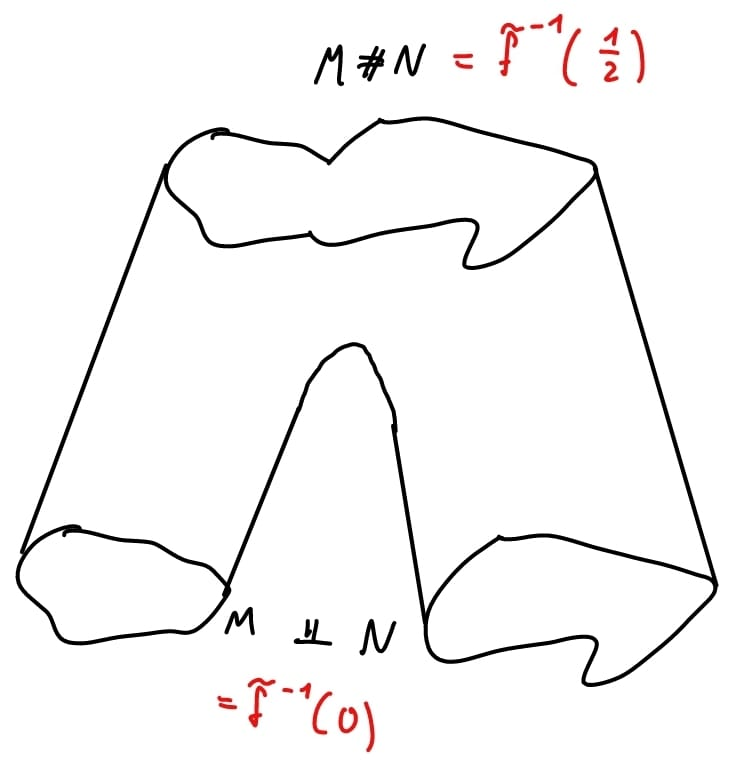
\includegraphics[width=0.4\textwidth]{pants.jpg}
    \end{center}
\end{example}
%Look this up again. Maybe it suffices to take \(X\) path-connected. Draw a picture.\\
%Probably to do: separating function. No

\begin{example}\label{points}
    \(\{\mathrm{pt}\}\) and \(\{\mathrm{pt}\}\dis\{\mathrm{pt}\}\) are not bordant, as \(1\)-manifolds either have 2 or 0 boundary points. Compact \(1\)-manifolds can be classified up to homeomorphism as the circle \(S^1\) (no boundary) and the interval \([0,1]\) (two boundary points). \unsure{reference}
\end{example}

\begin{remark}
     It follows that an odd number of points is never nullbordant as a singular manifold in \(\{\pt\}\), but an even number of points is. (This gives us \(\N_0(\pt)\cong\F_2\), as we will see later.)
\end{remark}


\begin{proposition}\cite[II, Satz 1.4]{brocker}\label{equivalence bordant}
    Being bordant is an equivalence relation on the set of closed singular manifolds.
\end{proposition}

\begin{proof}\cite{brocker},\ \cite[p.8]{conner}
    \begin{itemize}
        \item Symmetry: 
        Follows from the symmetry of the disjoint union. 
        If \((M,f)\) and \((N,g)\) are bordant, then there exists a nullbordism of \((M,f)+(N,g)=(M\dis N, f\dis g) = (N\dis M, g\dis f) = (N,g)+ (M,f)\). 
        So, a bordism between \((M,f)\) and \((N,g)\) is also bordism between \((N,g)\) and \((M,f)\).

        \item Reflexivity: 
        We have already constructed a bordism between \((M,f)\) and itself in example\ \ref{cylinder bordism}.

        \item Transitivity: 
        Let \((B_1,F_1)\) be the bordism between \((M_1,f_1)\) and \((M_2,f_2)\), and let \((B_2,F_2)\) be the bordism between \((M_2,f_2)\) and \((M_3,f_3)\). Then we can \enquote{glue} the two bordisms together at the common boundary \((M_2,f_2)\). 
        We only need to check that the gluing is smooth, i.e.\ \((B_1,F_1)\cup_{(M_2,f_2)}(B_2,F_2)\) is a smooth manifold. 
        By theorem\ \ref{collar}, we can find a collar of \(M_2\) in both \(B_1\) and \(B_2\). 
        %These collars glued together are homeomorphism to \(M_2\times(-1,1)\). This induces a smooth structure on the glued collar, and let \(B\setminus M_2\) inherit the smooth structure from \(B_1\) and \(B_2\). Then there exists a smooth structure on \(B\) by a previous lemma.
        Both these collars have the induced smooth structure of \(M_2\times [0,1)\). 
        Gluing the bordisms along \(M_2\) glues the collars to something diffeomorphic to \(M_2\times (-1,1)\), as the smooth structures align in the collars. 
        Since smoothness is local and we now have that the gluing is smooth for a open neighbourhood of \(M_2\), the whole gluing is smooth.
        \begin{center}
            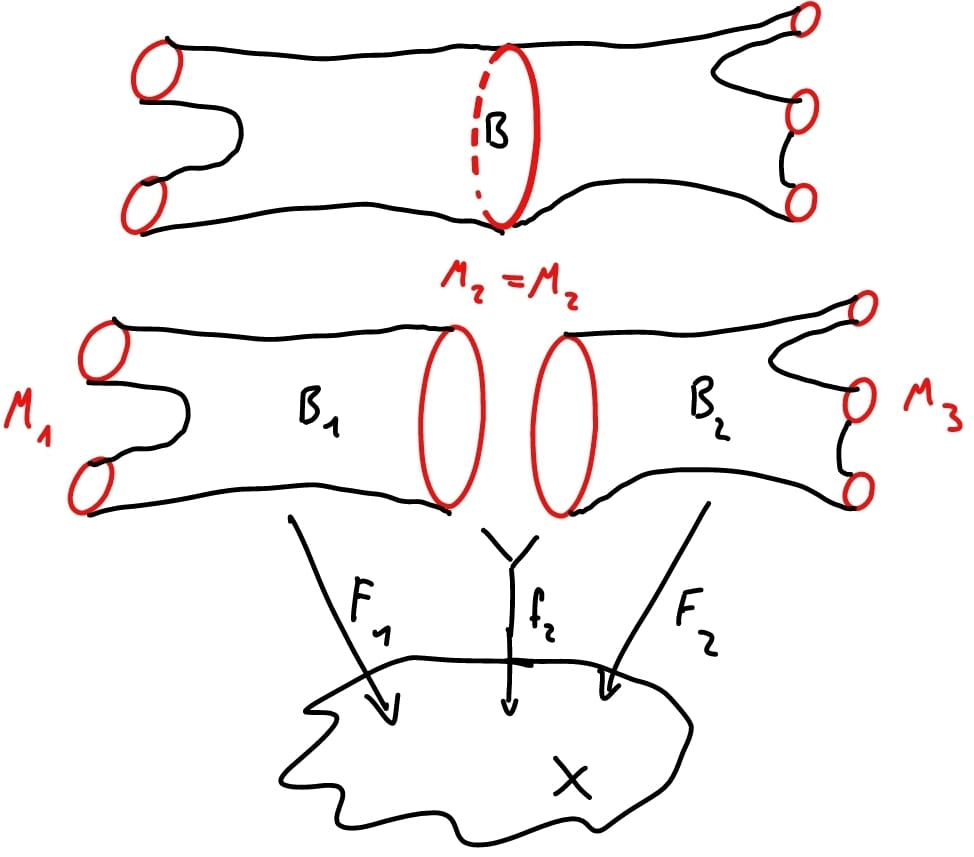
\includegraphics[width=0.4\textwidth]{transitivity.jpg}
        \end{center}
    \end{itemize}
\end{proof}
%Draw a picture. Done
%Need to add collar theorem somewhere up. Done (without proof)
%and inducing structure. No

\begin{remark}
    We required the singular manifolds to be closed, because on manifolds with non-empty boundary the bordism relation does not make sense, as they cannot be the boundary of another manifold (see theorem\ \ref{boundary manifold}).
\end{remark}

\begin{definition}[bordism group\ {\cite[II, Definition 1.5]{brocker}}]
    The equivalence classes of the bordism relation are called \demph{bordism classes}. 
    The bordism class of \((M,f)\) is denoted by \([M,f]\). 
    The set of bordism classes of \(n\)-dimensional singular manifolds in \(X\) is denoted by \(\mathfrak{N}_n(X)\) and is called the \(n\)\demph{-th bordism group of }\(X\).
    \[\mathfrak{N}_n(X)=\{\text{closed singular \(n\)-manifolds in \(X\)}\}\big/\text{bordism}\]
\end{definition}

\begin{observation}
    This might seem similar to the definition of singular homology groups. They were also defined by the quotient of the kernel by the image of a boundary map.
    In our case, the boundary map is \(\partial\), defined in definition\ \ref{singular manifold}. Let us introduce an index for this map to denote the dimension: \(\partial_n:\{n\text{-manifolds}\}\to\{\text{closed }(n-1)\text{-manifolds}\}\).
    Then: \[\N_n=\ker(\partial_n)\big/\im(\partial_{n+1})\]
\end{observation}
%Observe the similarity with the definition of singular homology groups: We defined the singular homology groups as the quotient of kernel and image of some maps. Here, the same thing happens: Our map here is the boundary map.

This notion only makes sense if we have an neutral element, so we can speak of a kernel. This is given by an abelian structure given in the next theorem. 

\begin{theorem}[{\cite[II, Satz 2.1]{brocker}}]\label{group structure}
    The bordism groups are abelian groups with the operation \(+\) defined in definition\ \ref{bordant}:
    \[[M_1,f_1]+[M_2,f_2]=[M_1+M_2,(f_1,f_2)]\]
    Every element in this group has order at most \(2\), making \(\mathfrak{N}_n(X)\) a \(\mathbb{F}_2\)-vector space.
\end{theorem}

\begin{proof}
    \ \cite{brocker}
    The neutral element is the bordism class of the empty manifold (i.e.\ the class of all nullbordant manifolds).\\
    \enquote{+} is associative and commutative, because the disjoint union is associative and commutative.\\
    It is well-defined:
    Let \((M_1,f_1),(M_1^\prime,f_1^\prime)\in[M_1,f_1]\), and \((M_2,f_2),(M_2^\prime,f_2^\prime)\in[M_2,f_2]\).
    Moreover, let \((B_1,F_1)\) and \((B_2,F_2)\) be bordisms between \((M_1,f_1)\) and \((M_1^\prime,f_2^\prime)\), respectively between \((M_2,f_2)\) and \((M_2^\prime,f_2^\prime)\). Then, a bordism between \((M_1,f_1)+(M_2,f_2)\) and \((M_1^\prime,f_1^\prime)+(M_2^\prime,f_2^\prime)\) is given by \((B_1,F_1)+(B_2,F_2)\). \todo{maybe more}\\
    Since being bordant is reflexive, every element is its own inverse.
\end{proof}

\begin{definition}[Product map\ {\cite[pp.12-13]{brocker}}]
    Let \(X,Y\) be two topological spaces. Then we define a product map
    \[\cdot:\mathfrak{N}_p(X)\times\mathfrak{N}_q(Y)\to\mathfrak{N}_{p+q}(X\times Y)\]
    as
    \[([M,f],[N,g])\mapsto [M\times N,f\times g]\]
\end{definition}

\begin{observation}
    This map is well defined, as for two bordant singular manifolds \((M,f)\) and \((M^\prime,f^\prime)\) with bordism \((B,F)\), we get a bordism between \((M\times N,f\times g)\) and \((M^\prime\times N, f^\prime\times g)\) by \((B\times N, F\times g)\). 
    This map is also bilinear (as a map between \(\F_2\)-vector spaces). Scalar multiplication is defined as \(0\cdot[M,f]=[\emptyset,\emptyset\to X]\), \(1\cdot[M,f]=[M,f]\). As \([\emptyset]\cdot[N,g]=[\emptyset]=[M,f]\cdot[\emptyset]\), we conclude for any \(a\in\F_2\): \([M,f]\cdot(a\cdot[N,g])=a\cdot([M,f]\cdot[N,g])=(a\cdot[M,f])\cdot[N,g]\). Additivity follows, as addition is defined as disjoint union: 
    \begin{align*}
        ([M,f]+[M',f'])\cdot[N,g]&=[M+M',(f,f')]\cdot[N,g]\\
        &=[((M+M')\times N ),(f,f')\times g]\\
        &= [(M\times N) + (M'\times N),(f\times g,f'\times g)]\\
        &=[M,f]\cdot[N,g]+[M',f']\cdot[N,g]\end{align*}
    %For \(a,b\in\F_2\), \([M,f],[M^\prime,f^\prime]\in\N_p(X)\) and \([N,g],[N^\prime,g^\prime]\in\N_q(Y)\):
    %\[([M,f]+a[M^\prime,f^\prime])\cdot([N,g]+b [N^\prime,g^\prime])\]
\end{observation}

%\begin{remark}
%    Check: Well-definedness, bilinearity
%\end{remark}

\noindent\textit{Notation.} For \(X=\{\mathrm{pt}\}\), we will write \(\mathfrak{N}_n\) for \(\mathfrak{N}_n(X)\) and for elements of \(\mathfrak{N}_n\), we will omit the map from the notation (\([M]=[M,f]\)).

\begin{definition}[graded bordism ring\ {\cite[Satz 2.2]{brocker}}]\label{bordism ring}
    \[\mathfrak{N}_\ast:=\bigoplus_{n\in\mathbb{Z}}\mathfrak{N}_n\]
    is a \(\Z\)-graded ring over \(\mathbb{F}_2\) via \(+\) and \(\cdot\) and is called the \demph{bordism ring}.
\end{definition}

\begin{remark}
    As \(\mathbb{F}_2\) is a field, \(\mathfrak{N}_\ast\) is a graded vector space over \(\mathbb{F}_2\).
\end{remark}

%Maybe do a quick check.

\begin{definition}[graded bordism module\ {\cite[Satz 2.3]{brocker}}]\label{bordism module}
    \[\mathfrak{N}_\ast(X):=\bigoplus_{n\in\mathbb{Z}}\mathfrak{N}_n(X)\]
    is a \(\Z\)-graded module over \(\mathfrak{N}_\ast\). It is called the \demph{bordism module}. Explicitly, the product map acts as follows:
    \[[M]\cdot[N,f]=[M\times N, f\circ \mathrm{pr}_2]\]
    where \(\mathrm{pr}_2:M\times N\to N\) is the projection onto the second factor.\\
    This is well-defined by the above observation.
\end{definition}

\begin{remark}
    Notice that in this definition, this is a left module, but since we could just project to the first factor instead, we also get a right module structure.
\end{remark}

\subsubsection{The Eilenberg-Steenrod Axioms}\label{es axioms}
The Eilenberg-Steenrod axioms are a set of axioms that characterize homology and cohomology theories.

\begin{definition}[Homology theory\ {\cite[\nopp I.3]{eilenberg}}, {\cite[Definition 1.1.]{luck}}]\label{homtheo}
    An \demph{ordinary homology theory} \(\mathcal{H}_\ast=(\mathcal{H}_\ast,\partial_\ast)\) with coefficients in \(R\)-modules is a covariant functor\[\mathcal{H}_\ast:\mathrm{TOP}^2\to\mathbb{Z}\text{-graded }R\text{-modules}\]
    together with a natural boundary operator 
    \[\partial_\ast:\mathcal{H}_\ast\to\mathcal{H}_{\ast-1}\circ I\]
    where \(I\) is a forgetful functor \(I:\mathrm{TOP}^2\to\mathrm{TOP}^2\), given by \(I(X,A)=(A,\emptyset)\). We will often write \(X\) for \((X,\emptyset)\) for any space \(X\).\\
    \(\mathcal{H}_\ast\) has to satisfy the following \demph{Eilenberg-Steenrod axioms for homology theories}:
    \begin{itemize}
        \item \textbf{Homotopy invariance}\\
        Let \(f,g:(X,A)\to(Y,B)\) be homotopic maps. Then for all \(n\in\mathbb{Z}\), we have
        \[\mathcal{H}_n(f)=\mathcal{H}_n(g):\mathcal{H}_n(X,A)\to\mathcal{H}_n(Y,B)\]
        \item \textbf{Long exact sequence}\\
        Let \((X,A)\) be a pair of spaces. Then for all \(n\in\mathbb{Z}\), we have the long exact sequence of homology groups:
        \begin{align*}
            \dots\xrightarrow{\partial_{n+1}(X,A)}\mathcal{H}_n(A)\xrightarrow{\mathcal{H}_n(i)}\mathcal{H}_n(X)\xrightarrow{\mathcal{H}_n(j)}\mathcal{H}_n(X,A)\xrightarrow{\partial_n(X,A)}\mathcal{H}_{n-1}(A)\to\dots
        \end{align*}
        \item \textbf{Excision}\\
        Let \(A\subset B\subset X\) be subspaces of \(X\) such that \(\overline{A}\subset B^\circ\). Then the inclusion \(i:(X\setminus B,A\setminus B)\to(X,A)\) induces an isomorphism of homology groups for all \(n\in\mathbb{Z}\):
        \[\mathcal{H}_n(i):\mathcal{H}_n(X\setminus A, B\setminus A)\xrightarrow{\cong}\mathcal{H}_n(X,B)\]
        \item \textbf{Dimension axiom}\\
        For the point space \(\mathrm{pt}\), we have
        \[\mathcal{H}_n(\mathrm{pt})\cong\begin{cases}R&n=0\\\{0\}&n\neq0\end{cases}\]
    \end{itemize}
\end{definition}

The following axiom is often considered part of the Eilenberg-Steenrod axioms, although it was formulated by Milnor 10 years later

\begin{itemize}
    \item \textbf{Disjoint union axiom}\ \cite[p.337, Additivity axiom]{milnor},\cite[Definition 1.1.]{luck}\\
        Let \({\{X_i\}}_{i\in I}\) be a family of topological spaces. Let \(j_i:X_i\to\coprod_{i\in I}X_i\) be the inclusion. Then for all \(n\in\mathbb{Z}\), we have a bijection:
        \[\bigoplus_{i\in I}\mathcal{H}_n(j_i):\bigoplus_{i\in I}\mathcal{H}_n(X_i)\xrightarrow{\cong}\mathcal{H}_n\left(\coprod_{i\in I}X_i\right)\]
\end{itemize}

The motivation behind the disjoint union axiom is the following uniqueness theorem.

\begin{theorem}[{\cite[p.340, Uniqueness Theorem]{milnor}}]
    Let \(\mathcal{H}_\ast\) be an ordinary homology theory satisfying the disjoint union axiom on CW-complexes with values in \(R\). Then there is a natural isomorphism \(\mathcal{H}_\ast\xrightarrow{\cong}H_\ast\), where \(H_\ast\) denotes singular homology.
\end{theorem}

A proof can be found in\ \cite{milnor}, but we will not need this here.

\begin{remark}
    If a functor only fails to satisfy the dimension axiom from definition\ \ref{homtheo}, it is called an \demph{extraordinary homology theory}.
\end{remark}


\subsubsection{Relative Bordism}

As homology theories are defined as functors from \(\mathrm{TOP}^2\), we will extend the definition of bordism to pairs of topological spaces.

\begin{definition}[relative bordism\ {\cite[pp.524-525]{dieck}}]
    For a pair of topological spaces \((X,A)\), we call \((M,f)=(M,\partial M,f)\) a \demph{singular manifold in }\((X,A)\), if \(f:(M,\partial M)\to (X,A)\) is a continuous map of pairs.\\
    Two \(n\)-dimensional singular manifolds \((M_0,f_0)\) and \((M_1,f_1)\) in \((X,A)\) are called \demph{bordant}, if there exists an (\(n+1\))-dimensional singular manifold \((B,F)\) in \(X\), such that:
    \begin{itemize}
        %\item \((B,F)\) is a (\(n+1\))-dimensional compact manifold with boundary,
        \item \(\partial B\) can be decomposed as  \(\partial B=M_0\cup M_1\cup M'\), where \(M_0,M_1,M'\) are considerd as embedded submanifolds of \(B\) with boundary, such that 
        \(\partial M'=\partial M_0\dis \partial M_1\), 
        \(M_i\cap M'=\partial M_i\) and \(\partial M_0
        \cap\partial M_1=\emptyset\), for \(i\in\{0,1\}\).

        \item \(\partial F\restrict{M_i}=f_i\), for \(i\in\{0,1\}\)

        \item \(F(M')\subseteq A\)
    \end{itemize}
    As before, \((B,F)\) will be called a \demph{bordism} between \((M_0,f_0)\) and \((M_1,f_1)\) and a \demph{nullbordism} of \((M_0,f_0)\) if \(M_1=\emptyset\).
\end{definition}

\begin{remark}
    If we take \(A=\emptyset\), we get the definition of (absolute) bordism as we had before. In particular, if \((M,f)\) and \((N,g)\) are bordant in the absolute sense, then they are also bordant in the relative sense with the same bordism (but there may be more possible bordisms in the relative sense).
\end{remark}

\begin{remark}
    Now, the bordism relation also makes sense for manifolds with non-empty boundary.
\end{remark}

\begin{example}\label{pokeball}
    Consider the disk \((D^n,f)\) as a singular manifold in \((X,A)\). 
    %We already know that \((D^n\times [0,1],f\circ\mathrm{pr}_1)\) is a bordism between \((D^n,f)\) and itself. 
    We have a bordism \(B,F\) between \((D^n,f)\) and itself by \(B=D^{n+1}\). We have to cover \(\partial D^{n+1}=S^n\) by two \(D^n\)s and \(M^\prime\), which can be done by taking almost all of each the upper and the lower hemisphere as \(D^n\) 
    \todo{(In this example, the chosen embedding heavily matters. We will embed them such that there is only one pair of points such that the antipodal points in the embedding correspond to each other.)} 
    and the remaining cylinder around the equator as \(M'\). 
    Now \(F\) just has to map \(M'\) to \(A\) (and along with it, also \(\partial M_0\) and \(\partial M_1\), as desired). 
    To do this, \(F\) \enquote{squeezes} the disk such that the \(D^n\)s are identified together and then maps the resulting disk with the remains of \(M'\) to \((D^n,\partial D^n)\) via the identity on \(D^n\) and contracting \(M'\) to its boundary. Lastly, apply \(f\).
    \begin{center}
        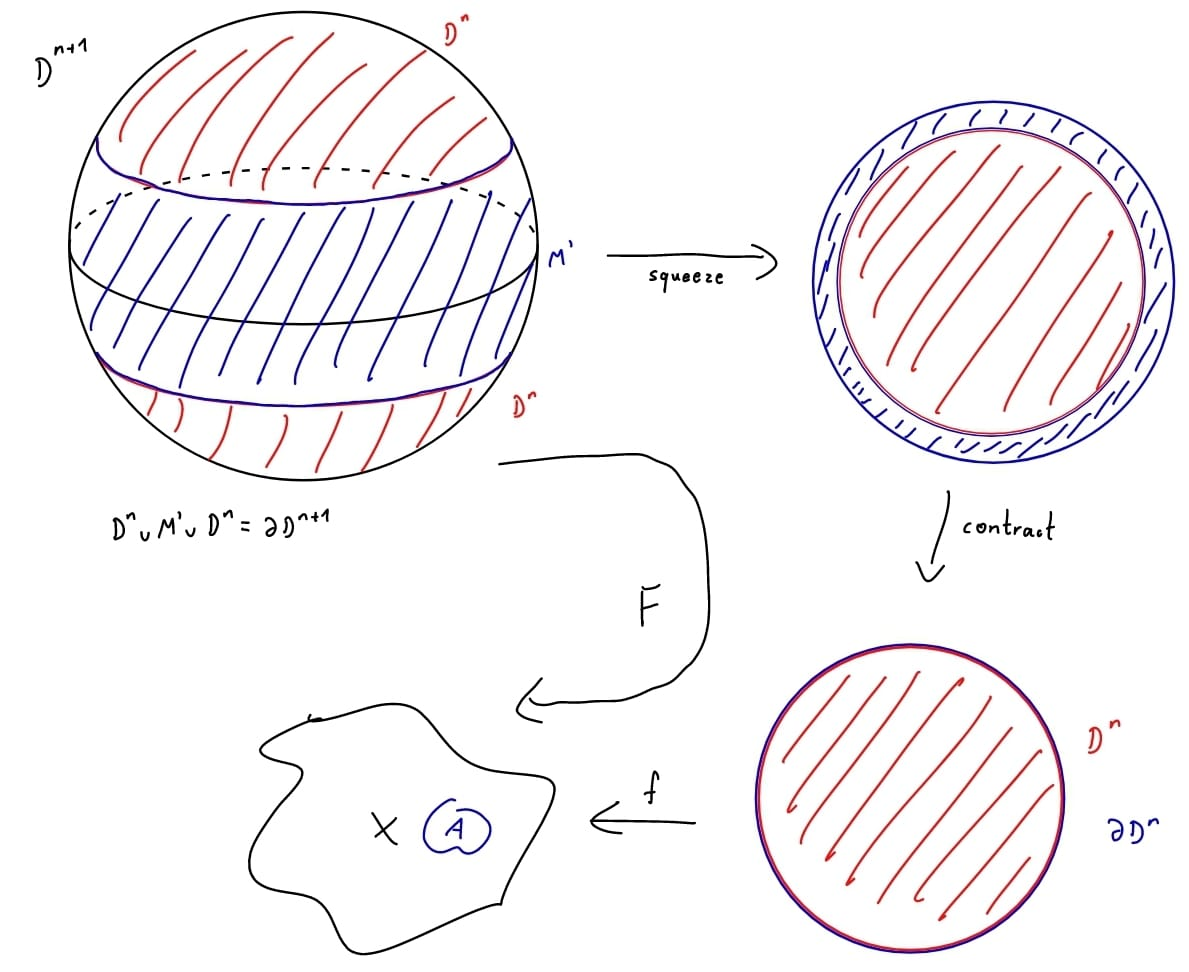
\includegraphics[width=0.6\textwidth]{squeeze2.jpg}
    \end{center}
\end{example}

\begin{remark}
    The above example is just the same as the cylinder bordism in example\ \ref{cylinder bordism}, if we had constructed it as a cylinder we would not have had to worry about the embedding. If cylinder bordism works for manifolds with non-empty boundary, we can take its lateral surface (\(=\partial M_0\times [0,1]\)) as \(M'\). For this to work, it has to be shown that \(M\times[0,1]\) admits a smooth structure; a priori it is a manifold with corners. This is done by applying a technique called \demph{straightening the angle}\ \cite[I.3]{conner}. We will not go into detail here, but the main idea is to find an submanifold of codimension 2 containing all corners and a open neighbourhood of it which can be charted into \(\R^{n-2}\times\R_{\geq0}^2\) and then getting new charts by composing with a diffeomorphism \(\R_{\geq0}^2\xrightarrow\cong\R\times\R_{\geq0}\).
\end{remark}

\begin{theorem}[{\cite[p.525]{dieck}}]
    Relative bordism is an equivalence relation on the set of singular manifolds in \((X,A)\).
\end{theorem}

\begin{proof}
    The proof is similar to the proof of proposition\ \ref{equivalence bordant}. 
    Symmetry is clear, for reflexivity, we now also have the cylinder as stated in the above remark. 
    For transitivity, we again glue the bordisms along their common boundary \(M_2\), but as \(M_2\) may have boundary now, we glue the bordism along an open neighbourhood \(U\) (in \(\partial B_1\) and \(\partial B_1\)) of \(M_2\). 
    To see that this is smooth, we again look at the collars of \(\partial B_i\). This time we restrict the collars to \(U\) and see that the collars are diffeomorphic to \(M_2\times(-1,1)\). The rest of the proof is the same as in proposition\ \ref{equivalence bordant}. \todo{maybe more}
\end{proof}

Relative bordism groups are also defined to be the set of relative bordism classes, analogously to absolute bordism groups, but as manifolds with boundary are also allowed now, we have
\[\N_n(X,A)=\{\text{\textit{compact} singular $n$-manifolds in $(X,A)$}\}\big/\text{relative bordism}.\]
These also are abelian by the same proof (theorem\ \ref{group structure}). The product map is defined as \[\cdot:\N_p(X,A)\times\N_q(Y,B)\to\N_{p+q}(X\times Y, (A\times Y)\cup(X\times B))\]
on elements, it does the same as before. A product of manifolds is again a smoothable manifold by straightening the angle as in the remark after example\ \ref{pokeball}. Again, we get a graded module structure
\[\N_\ast(X,A):= \bigoplus_{n\in\Z}\N_n(X,A)\]
over \(\N_\ast\), the relative bordism module.

\begin{lemma}[{\cite[VIII, Lemma 13.10]{tomdieck}}]\label{almost excision} %\cite[Lemma 5.1]{zhang} \cite[Lemma 21.1.8]{dieck}
    Let \([M,f]\in\mathfrak{N}_n(X,A)\) and \(N\) an \(n\)-dimensional submanifold of \(M\). 
    Suppose that \([N,f\restrict{N}]\in\mathfrak{N}_n(X,A)\) and \(f(M\setminus N)\subseteq A\). 
    Then \([M,f]=[N,f\restrict{N}]\) in \(\mathfrak{N}_n(X,A)\).
\end{lemma}

\begin{proof}\cite{tomdieck}
    We need to show that \((M,f)\) and \((N,f\restrict{N})\) are bordant.\\
    Let \(B=M\times [0,1]\) the cylinder.\ \(\partial B= M\times\{0\}\cup M\times\{1\}\cup \partial M\times I\). Define \(F:B\to X\) as \(F(p,t)=f(p)\).\\
    \textit{Claim:} \((B,F)\) is a bordism between \((M\times \{0\},f\circ\mathrm{pr}_1)\) and \((N\times \{1\}, f\restrict{N}\circ\mathrm{pr}_1)\).\\
    As both are embedded submanifolds of \(B\), we only need to check that \(\partial B\setminus((M\times \{0\})\cup (N\times\{1\}))\) is mapped into \(A\) by \(F\).
    \begin{align*}
        F(\partial B\setminus((M\times \{0\})\cup (N\times\{1\})))&\subseteq F((\partial M\times I)\cup ((M\times\{1\})\setminus (N\times \{1\})))\\
        =f(\partial M)\cup f(M\setminus N)&\subseteq A
    \end{align*}
    %\[g(\partial B\setminus(M_0\cup N_1))=g((M_1\setminus N_1)\cup(\partial M\times I))=f(M\setminus N)\cup f(\partial M)\subseteq A\]
\end{proof}

\subsubsection{Bordism Homology}

\begin{lemma}\cite[II, Satz 3.2]{brocker}\label{functoriality}
    Relative bordism is a covariant functor \[\mathfrak{N}_\ast:\mathrm{TOP}^2\to\text{graded \(\mathfrak{N}_\ast\)modules}\]
\end{lemma}

\begin{proof}\cite{brocker} 
    Let \((X,A)\in\mathrm{Ob}(\mathrm{TOP}^2)\), we already saw
    \[(X,A)\xmapsto{\mathfrak{N}_\ast}\mathfrak{N}_\ast(X,A)\]
    For a map \(\mathrm{Mor}(\mathrm{TOP}^2)\ni f:(X,A)\to(Y,B)\), we take the induced map on the bordism groups:
    \[f_\ast:=\mathfrak{N}_\ast(f):\mathfrak{N}_\ast(X,A)\to\mathfrak{N}_\ast(Y,B)\]
    given by 
    \[f_\ast[M,g] = [M,f\circ g]\]
    %\(f_\ast[M,g]=[M,f\circ g]\) for \([M,g]\in\mathfrak{N}_n(X,A)\) and \(n\in\mathbb{N}\).\\
    Then we get that \(\mathfrak{N}_\ast(\mathrm{id}_{(X,A)})=\mathrm{id}_{\mathfrak{N}_\ast(X,A)}\) and for \(f:(X,A)\to(Y,B), g:(Y,B)\to(Z,C)\), we have for any \([M,h]\in\mathfrak{N}_\ast(X,A)\):
    \[{(g\circ f)}_{\ast}[M,h]=[M,g\circ f\circ h]=g_\ast[M,f\circ h]=g_\ast\circ f_\ast[M,h]\]
\end{proof}

The boundary map is defined similarly as before.
\[\partial_n:\N_n(X,A)\to\N_{n-1}(A,\emptyset)\]
\[\partial_n(M, f)=(\partial M,f\restrict{\partial M})\]

\begin{lemma}[Naturality of the boundary map]\label{naturality}
    The following diagram commutes for any \(f:(X,A)\to(Y,B)\) and \(n\in\Z\): %(Diagrams cannot be compiled for some reason)
    \begin{center}
        \begin{tikzcd}
            {\mathfrak{N}_n(X,A)} \arrow[r, "\partial_n"] \arrow[d, "f_\ast"'] & {\mathfrak{N}_{n-1}(A)}  \arrow[d, "{\left(f\restrict{A}\right)}_\ast"] \\
            {\mathfrak{N}_n(Y,B)} \arrow[r, "\partial_n"]  & {\mathfrak{N}_{n-1}(B)}
        \end{tikzcd}
    \end{center}
\end{lemma}

\begin{proof}
    Let \([M,g]\in\mathfrak{N}_n(X,A)\).\ \(\partial_n[M,g]=[\partial M, g\restrict{\partial M}]\in\N_{n-1}(A)\), as \(\partial M\) is closed and \(g\) maps \(\partial M\) to \(A\). % maps this to \([\partial M,g\restrict{\partial M}]\in\mathfrak{N}_{n-1}(A)\).
    Now \({f\restrict{A}}_\ast([\partial M,g\restrict{\partial M}])=[\partial M,f\circ g\restrict{\partial M}]\in \mathfrak{N}_{n-1}(B)\).\\
    On the other side, \((\partial_n\circ f_\ast)[M,g]=\partial_n [M,f_\ast\circ g]=[\partial M,(f\circ g)\restrict{\partial M}]\in \mathfrak{N}_{n-1}(B)\), which is the same as the previous composition, hence,
    \[\partial_n\circ f_\ast={f\restrict{A}}_\ast\circ \partial_n\]
    and the diagram commutes.
\end{proof}

\begin{lemma}[Homotopy invariance]\cite[II, Satz 3.1]{brocker}\label{htpy inv}
    \(\mathfrak{N}_\ast\) is homotopy invariant.
\end{lemma}

\begin{proof}\cite{brocker}\cite[Chapter I, 5.5]{conner}
    Let \(f,g:(X,A)\to(Y,B)\) be homotopic maps of pairs. Let \(h:(X\times I,A\times I)\to (Y,B)\) be a homotopy between \(f\) and \(g\). Then, for \([M,F]\in\N_\ast(X,A)\), we have a bordism between \(f_\ast[M,F]\) and \(g_\ast[M,F]\) by the cylinder \((M\times I, h\circ (F\times\mathrm{id}_I))\).
\end{proof}

%Maybe an explanation in the end (\cite{conner}). No

%Maybe do an example here. (Special case Cylinder done before showing that bordism is an equivalence relation) No

\begin{remark}%\cite[I.5, pp.12-13]{conner}
    For a closed manifold \(M\) with \([M,f]=0\in\N_n(X,A)\) and a nullbordism \((B,F)\) of \((M,f)\). Then \(\partial B\setminus M\) is a closed \(n\)-dimensional submanifold of \(B\). For a proof, see \cite[Lemma 5.4]{zhang}.
\end{remark}

\begin{lemma}[Long exact sequence\ {\cite[Proposition 21.1.9]{dieck}}]\label{les}
    \(\mathfrak{N}_\ast\) satisfies the long exact sequence axiom.
\end{lemma}

%Compare with\ \cite{zhang}!

\begin{proof}\cite{dieck}
    Let \(i,j\) be the inclusion maps \(i:A\to X, j:X=(X,\emptyset)\to(X,A)\).\\
    \textit{Claim:} The sequence
    \[\dots\xrightarrow{\partial_{n+1}}\mathfrak{N}_n(A)\xrightarrow{i_\ast}\mathfrak{N}_n(X)\xrightarrow{j_\ast}\mathfrak{N}_n(X,A)\xrightarrow{\partial_n}\mathfrak{N}_{n-1}(A)\xrightarrow{i_\ast}\dots\]
    is exact.
    \begin{itemize}
        \item \textbf{Exactness at \(\mathfrak{N}_n(A)\):}
        \(i_\ast\circ \partial=0\), as for \([M,f]\in\N_{n+1}(X,A)\), \(\partial_{n+1} [M,f]=[\partial M,f\restrict{\partial M}]\), which, considered as an element in \(\N_n(X)\) is nullbordant via the nullbordism \((M,f)\).

        Let \((M,f)\in\N_n(A)\) with nullbordism \((B,F)\) in \(X\). Then, \(\partial_{n+1}[B,F]=[M,f]\).

        \item \textbf{Exactness at \(\mathfrak{N}_n(X)\):} Let \([M,f]\in\mathfrak{N}_n(A)\). Choose \(N=\emptyset\) and use lemma\ \ref{almost excision} to get \([M,f]=0\) in \(\mathfrak{N}_n(X,A)\), so \(j_\ast\circ i_\ast=0\).
        
        Now let \([M,f]\in\ker(j_\ast)\subseteq \mathfrak{N}_n(X)\). Then there exists a singular manifold \((B^{n+1},F)\) in \((X,A)\) of \([M,f]\). \((B,F)\) is a bordism between \(M,f\) and \(\partial B\setminus M,F\restrict{\partial B\setminus M}\), as \(\partial B\setminus M\) is a closed submanifold of \(B\) by the previous remark. 
        Since \(F(\partial B\setminus M)\subseteq A\), \([\partial B\setminus M,F\restrict{\partial B\setminus M}]\in\N_n(A)\). So, \(i_\ast[\partial B\setminus M,F\restrict{\partial B\setminus M}]=[M,f]\in\N_n(X)\).

        \item \textbf{Exactness at \(\mathfrak{N}_n(X,A)\):} \(\partial \circ j_\ast=0\) holds because every element in \(\N_n(X)\) is a closed manifold, so it has empty boundary, hence applying the boundary map gets us to \([\emptyset,\emptyset\to X]\) which is the zero element in \(\N_{n-1}(A)\).
        
        Let \(\partial[M,f]=0\), and \([B,F]\) be a nullbordism of \([\partial M, f\restrict{\partial M}]\). Identify \((M,f)\) and \((B,F)\) along \(\partial M\). This is smooth by the same argument as in proposition\ \ref{equivalence bordant}. Call the resulting singular manifold \((C,g)\). This has no boundary, so \([C,g]\in\N_n(X)\) Now with lemma\ \ref{almost excision}, get \(j_\ast[C,g]=[M,f]\).
    \end{itemize}
\end{proof}


\begin{comment}[Transversality, Sard, Mayer-Vi\"etoris,...]
Before checking the next axioms, we need to do some more differential topology. (Maybe I will put this in chapter 1\dots)

\begin{definition}[Tangent space\ \cite{lee}]
\end{definition}

Need a few more things, differential, etc.

\begin{definition}[Transversality\ \cite{brocker}]
    Let \(f:M\to N\) a smooth map between manifolds. Let \(U\subseteq N\) be an (\(n-k\))-dimensional submanifold of \(N\) 
\end{definition}
Maybe Lee's definition is better.\\

\begin{definition}[Regular value]
\end{definition}

\begin{theorem}[Sard's theorem\ \cite{lee}]
\end{theorem}

I will not prove this theorem, a proof can be found in\ \cite{lee}.

\begin{definition}[Seperating function\cite{brocker}]
\end{definition}

\begin{lemma}
    Slogan: The Mayer-Vi\"etoris sequence is equivalent to the excision axiom.
\end{lemma}

\begin{lemma}
    The Mayer-Vi\"etoris sequence
    \[\dots\xrightarrow{\partial}\mathfrak{N}_n(X_0\cap X_1)\xrightarrow{\alpha}\mathfrak{N}_n(X_0\oplus\mathfrak{N}_n(X_1))\xrightarrow{\beta}\mathfrak{N}_n(X)\xrightarrow{\partial}\mathfrak{N}_{n-1}(X_0\cap X_1)\xrightarrow{\alpha}\dots\]
    is exact.
\end{lemma}

\end{comment}

Only the excision axiom is left to check. To see the excision property, we need some preliminary lemmas.

\begin{lemma}[{\cite[Chapter I, 3.1]{conner}}]\label{plemma}%{\cite[Lemma 5.6]{zhang}}
    Let \(M^n\) be a compact manifold, let \(K,L\subseteq M\) closed, such that \(K\cap L=\emptyset\). Then there exists a closed \(n\)-dimensional submanifold \(N\subset M\) with boundary \(\partial N\) such that \(K\subseteq N\) and \(L\cap N=\emptyset\).
\end{lemma}

\begin{proof}\cite{conner}\\
    \(K\cap\partial M\) and \(L\cap\partial M\) are still disjoint, closed in \(\partial M\), so we can find disjoint closed subsets \(K',L'\subseteq\partial M\) such that \(K\subseteq\overset{\circ}{K'}\), \(L\subseteq\overset{\circ}{L'}\). 
    We find a collar \(C\) of \(\partial M\) by theorem\ \ref{collar} and identify it with \(\partial M\times[0,1)\). 
    As \(M\) is compact, there exists a \(t\in (0,1)\) such that \(L\cap (\partial M\times [0,t))\subseteq L'\) and \(K\cap (\partial M\times [0,t))\subseteq K'\). 
    Now \(M':=M\setminus (\partial M\times [0,t))\) is a closed \(n\)-dimensional submanifold of \(M\). By Urysohn's lemma\ \ref{urysohn}, there exists a smooth function \(\alpha:M'\to[0,1]\) such that \(\alpha\restrict{(K'\times \{t\})\cup (K\cap M')}=0\) and \(\alpha\restrict{(L'\times \{t\})\cup(L\cap M')}=1\). 
    We can extend \(\alpha\) to \(M\) by \(\alpha(p,s):=\alpha(p,t)\) for \(p\in \partial M\) and \(s\in[0,t)\). 
    By theorem\ \ref{sard}, there is a regular value \(r\in(0,1)\) of \(\alpha\). 
    Then \(N:=\alpha^{-1}([0,r])=\alpha^{-1}(-\infty,r]\) is a \(n\)-dimensional closed submanifold of \(M\)%with boundary \(\partial N=\alpha^{-1}(r)\)
    . By construction, \(K\subseteq N\), \(L\cap N=\emptyset\).\\
    It remains to show that \(N\) is smoothable, but we will omit the proof here.
\end{proof}

%In the above (nonexistent yet, may look into Conner,Floyd) proof, a smooth \(\alpha\) with regular value \(r\) is constructed.

\begin{lemma}[{\cite[Lemma 5.8]{zhang}}]\label{plemma2}
    Let \(K,L,M,N,\alpha,r\) be as in lemma\ \ref{plemma}. Then,
    \[\partial N\subseteq \partial M\cup \alpha^{-1}(r)\subseteq \partial M\cup((M\setminus K)\cap(M\setminus L))\]
\end{lemma}

\begin{proof}\cite{zhang}
    \textit{First inclusion:} Assume \(p\in\partial N\setminus \partial M\). We need to show that \(\alpha(p)=r\). By assumption, \(p\) is an interior point of \(M\), so we can find a euclidean neighbourhood \(U\) of \(p\) in \(M\). 
    As \(p\in N\), \(\alpha(p)\leq r\). Suppose \(\alpha(p)<r\). Then, for a \(r'\in(\alpha(p),r)\), we have \(p\in\alpha^{-1}([0,r'))\subseteq N\). Since \(\alpha^{-1}([0,r'))\) is open in \(M\), it is open in \(N\) and \(U\cap V\) is an open euclidean neighbourhood of \(p\) in \(N\). But then, \(p\) is an interior point of \(N\), contradicting the assumption that \(p\in\partial N\). So, \(\alpha(p)=r\).\\
    \textit{Second inclusion:} Since \(\alpha\restrict{K}=0\) and \(\alpha\restrict{L}=1\), we have \(\alpha^{-1}(r)\subseteq M\setminus (K\cup L)\).
\end{proof}

\begin{lemma}[Excision axiom\ {\cite[Theorem 5.10]{zhang}}]\label{excision}
    Let \((X,A,Z)\) be a triple of topological spaces satisfying \(\overline{Z}\subseteq\overset{\circ}{A}\). Then the inclusion map \(i:(X\setminus Z,A\setminus Z)\hookrightarrow(X,A)\) induces an isomorphism of bordism groups:
    \[i_\ast:\mathfrak{N}_n(X\setminus Z,A\setminus Z)\xrightarrow{\cong}\mathfrak{N}_n(X,A)\]
\end{lemma}

\begin{proof}\cite{zhang}
    \textbf{Surjectivity}: Let \([M,f]\in\mathfrak{N}_n(X,A)\). Then the preimages \(K=f^{-1}(X\setminus\overset{\circ}A)\) and \(L=f^{-1}(\overline{Z})\) are disjoint and closed subsets of \(M\). By lemma\ \ref{plemma}, there exists a closed submanifold with boundary \(N\subset M\) such that \(K\subseteq N\) and \(L\cap N=\emptyset\).\\
    From \(L\cap N=\emptyset\), it follows that \(f(N)\subseteq X\setminus\overline{Z}\). By lemma\ \ref{plemma2}, we have \(\partial N\subseteq \partial M\cup((M\setminus K)\cap(M\setminus L))\). So, for any \(p\in \partial N\), we have either \(p\in\partial M\), implying \(f(p)\in A\), or \(p\in(M\setminus K)\), implying \(f(p)\in\overset{\circ}A\). In any case, we get \(f(\partial N)\subseteq A\setminus\overline{Z}\), so \([N, f\restrict{N}]\in\mathfrak{N}_n(X\setminus Z,A\setminus Z)\).\\
    As \(f^{-1}(X\setminus\overset{\circ}A)\), we get \(f(M\setminus N)\subseteq \overset{\circ}A\). By lemma\ \ref{almost excision}, we get \(i_\ast[N,f\restrict{N}]=[M,f]\).

    \noindent\textbf{Injectivity}: Take \([M,f]\in\mathfrak{N}_n(X\setminus Z, A\setminus Z)\) such that \(i_\ast[M,f]=0\) in \(\mathfrak{N}_n(X,A)\). Then there exists %an (\(n+1\))-manifold \(B\) and \(g:B\to X\), such that \(M\) is an embedded submanifold of \(\partial B\), \(g(\partial B\setminus M)\subseteq A\) and \(g\restrict{M}=f\).\\
    a nullbordism \((B,F)\) with \(F(\partial B\setminus M)\subseteq A\).\\
    Again, let \(K=F^{-1}(X\setminus\overset{\circ}A)\), \(L=F^{-1}(\overline{Z})\). By lemma\ \ref{plemma}, we have a submanifold \(N^{n+1}\subseteq B\) such that \(K\subseteq N\), \(N\cap L=\emptyset\). Then, \([\partial N,F\restrict{\partial N}]\in\mathfrak{N}_n(X\setminus Z, A\setminus Z)\) nullbordant by \((N,F\restrict{N})\).\\
    \emph{Claim}: \(M\cap\partial N=M\cap N\).\\
    \enquote{\(\subseteq\)} is clear. For \enquote{\(\supseteq\)}, take \(p\in M\cap N\). Then \(p\in\partial B\), so there exists a chart \(\varphi:U\to\mathbb{H}^{n+1}\) of \(B\), such that \(\varphi(p)\in\partial\mathbb{H}^{n+1}\). So, \(p\in\partial N\).\\
    Then \(M\cap\partial N\) is an submanifold of \(M\), because
    \begin{equation}\label{*}
        M\cap\partial N= M\cap N={(\alpha\restrict{M})}^{-1}([0,r]),\tag{$\star$}
    \end{equation}
    where \(\alpha\) is again such that \(N=\alpha^{-1}([0,r])\). 
    By theorem\ \ref{sard}, we assume that \(r\) is also a regular value of \(\alpha\restrict{M}\). Now we see that \([M\cap\partial N,f\restrict{M\cap\partial N}]\in\mathfrak{N}_n(X\setminus Z,A\setminus Z)\): \(f(M\cap\partial N)\subseteq f(M)\subseteq X\setminus Z\) and \(f(\partial(M\cap\partial N))\subseteq A\setminus Z\) because of\ (\ref{*}) and lemma\ \ref{plemma2}, as \(\partial(M\cap\partial N)\subseteq\partial M\cup(B\setminus (K\cup L))\).\\
    \textit{Claim}: 
    \([M,f]=[M\cap N,f\restrict{M\cap N}]\in\mathfrak{N}_n(X\setminus Z,A\setminus Z)\). \\
    By lemma\ \ref{almost excision}, it is enough to show that 
    \(f(M\setminus(M\cap N))=f(M\setminus M\cap \partial N)\subseteq A\setminus Z\). 
    Let \(p\in M\setminus\partial N=M\setminus N\), then \(f(p)\in X\setminus Z\) because \(p\in M\), and \(f(p)\in A\), because \(p\notin N\).\\
    By exactly the same argument, \([M\cap N,f\restrict{M\cap N}]=[\partial N,F\restrict{\partial N}]\in\mathfrak{N}_n(X\setminus Z,A\setminus Z)\). 
    Since \(M\cap N\) is an submanifold of \(M\), it is also an submanifold of \(\partial N\). 
    Now, we only need to show that \(F(\partial N\setminus(M\cap N))=F(\partial N\setminus M)\subseteq A\setminus Z\). 
    We know \(\partial N\subseteq\partial B\cup(B\setminus(K\cup L))\) (lemma\ \ref{plemma2}). 
    Let \(p\in\partial N\setminus M\), then either \(p\in(B\setminus(K\cup L))\setminus M\) or \(p\in\partial B\setminus M\). In the first case, \(F(p)\in A\setminus Z\), so we are done. 
    In the second case, we know \(p\notin L\), because \(B\cap L=\emptyset\). So, \(F(p)\notin\overline{Z}\). By construction, we have \(F(\partial B\setminus M)\subseteq A\), so \(F(p)\in A\). \(\Rightarrow g(p)\in A\setminus Z\).\\
    In total, we have shown that \((M,f), (M\cap N,f\restrict{M\cap N}), (\partial N,F\restrict{\partial N})\) are bordant. All three are nullbordant, since \((\partial N,F\restrict{\partial N})\) is nullbordant in \(\mathfrak{N}_n(X\setminus Z,A\setminus Z)\) by \((N,F\restrict{N})\). Thus, \([M,f]=0\) in \(\mathfrak N_n(X\setminus Z,A\setminus Z)\).
\end{proof}

Now it already follows that bordism is a homology theory.\ \todo{But let's take a look at the other axioms too.}

\begin{lemma}[Disjoint union axiom\ {\cite[Theorem 5.3]{zhang}}]\label{disjoint union}
    The disjoint union axiom holds for bordism.
\end{lemma}

\begin{proof}\cite{zhang}
    We need to show that 
    \[\bigoplus_{i\in I}\mathfrak{N}_n(j_i):\bigoplus_{i\in I}\mathfrak{N}_n(X_i)\to\mathfrak{N}_n\left(\coprod_{i\in I}X_i\right)\] 
    is an isomorphism.\\
    \textit{Claim}: \[\iota:\bigoplus_{i\in I}[M_i,f_i]\mapsto \left[\coprod_{i\in I}M_i,\coprod_{i\in I} f_i\right]\]
    gives us the desired isomorphism.\\
    \textbf{Well-definedness}: All but finitely many \([M_i,f_i]\) are \(0\). Thus, \(\coprod M_i\) is a finite disjoint union of compact manifolds, so it is compact.\\
    \textbf{Injectivity}: Suppose \(\iota\left(\bigoplus_i[M_i,f_i]\right)=0\) in \(\mathfrak{N}_n(\coprod_i X_i)\). 
    Then there exists a nullbordism \((B,F)\) of it.\ \todo{\(B\) as a space is the disjoint union \(\coprod_i B_i:=\coprod_i F^{-1}(X_i)\), all of the \(B_i\) being open and closed in \(B\)}. 
    Thus, the \(B_i\) are compact \((n+1)\)-manifolds. Also, \(\partial(B_i,F\restrict{B_i})=(M_i,f_i)\), so all the \((M_i,f_i)\) are nullbordant and the sum \(\bigoplus[M_i,f_i]=0\).
    \\
    \textbf{Surjectivity}: Suppose \([M,f]\in\mathfrak{N}_n(\coprod_i X_i)\). As in the proof of injectivity, we can write \(M=\coprod_i M_i:=f^{-1}(X_i)\), with all \(M_i\) compact manifolds. Then a preimage of \([M,f]\) under \(\iota\) is \(\bigoplus[M_i,f\restrict{M_i}]\).
\end{proof}

\begin{observation}\label{dimension axiom}
    Bordism does not satisfy the dimension axiom.\\
    \textit{Check}: 
    Consider \([\R\mathbb{P}^2]\in \N_2\). 
    There is no \(3\)-manifold that has \(\mathbb{RP}^2\) as its boundary. 
    We can see this by the euler characteristic: \(\chi(\mathbb{RP}^2)=1\). 
    However boundaries of manifolds always have even euler characteristic\ \cite[Proposition 18.6.2]{dieck}. 
    So, \(\N_2\not\cong \{0\}\). 
    %Compute \(\mathfrak{N}_2\). We know a classification of compact \(2\)-manifolds. They are either homeomorphic to \(S^2\), \(\mathbb{T}^2\), \(\mathbb{RP}^2\) or a connected sum of these. We have already seen that \(S^2\) and \(\mathbb{T}^2\) are nullbordant. For \(\mathbb{RP}^2\), however, we have that \(\chi(\mathbb{RP}^2)=1\). But we have that boundaries of manifolds always have even euler characteristic {\cite[Proposition 18.6.2]{dieck}}, so \(\mathbb{RP}^2\) cannot be nullbordant and \(\mathfrak{N}_2\) cannot be \(0\).% In fact, \([\mathbb{RP}^2]\) is the generator of \(\mathfrak{N}_2\cong\mathbb{F}_2\)
    %this fact later
\end{observation}

%I could include a definition for the connected sum...

Now we can finally conclude:

\begin{theorem}
    Bordism defines a homology theory satisfying the disjoint union axiom.
\end{theorem}

\begin{proof}
    This follows directly from the lemmas\ \ref{functoriality},\ \ref{htpy inv},\ \ref{les},\ \ref{excision} and\ \ref{disjoint union}.\\
    %The only axiom that does not hold is the dimension axiom.\\
    As it is not an ordinary homology theory (i.e.\ the dimension axiom does not hold), we call bordism an \demph{extraordinary} or a \demph{generalized} homology theory.
\end{proof}


%This theorem should probably be done after cobordism.
%\begin{theorem}
%    There is a natural equivalence of homology theories
%    \[\mathfrak{N}_\ast(--)\xrightarrow{\cong}\mathcal{H}_\ast(--,\mathbf{MO})\]
%\end{theorem}

\subsubsection{Calculations}

%We will now calculate the bordism groups.

As we have already noted in example\ \ref{points}, we have \(\N_0\cong\F_2\). An even number of points is nullbordant, an odd number is not. Let us try to argue for higher dimensions.\\
The only closed \(1\)-dimensional manifold (up to diffeomorphism) is \(S^1\). As \(S^1=\partial D^2\), we conclude \(\N_1\cong \{0\}\).\\
Closed \(2\)-manifolds are classified to be \(S^2, \#_i\T^2, \#_i\mathbb{RP}^2\). I.e.\ they are classified by euler characteristic and orientability. We know \(S^2=\partial D^3\) and \(\T^2=\partial (S^1\times D^2)\). So \(\#_i\T^2=\partial(\#_i D^3)\). From the above observation, we know \(\mathbb{RP}^2\) is not nullbordant. 
By example\ \ref{pants}, we have \([\mathbb{RP}^2\#\mathbb{RP}^2]=[\mathbb{RP}^2]+[\mathbb{RP}^2]\), and by proposition\ \ref{equivalence bordant}, this is \([\mathbb{RP}^2]+[\mathbb{RP}^2]=0\). Inductively, any even number of connected sums of \(\mathbb{RP}^2\)s is nullbordant, and any odd number of connected sums of \(\mathbb{RP}^2\)s is not nullbordant, but in the same equivalence class as \(\mathbb{RP}^2\). So we have \(\N_2\cong\F_2\) with \(\mathbb{RP}^2\) as generator.\\
%\(\mathbb{RP}^2\#\mathbb{RP}^2\) is homeomorphic to the Klein bottle \(K=(S^1\times [0,1])\big/((x,0)\sim (-x,1))\), where \(S^1\) is described as \([-1,1]\big/ (-1\sim 1)\). \(K\) is nullbordant by \(K=\partial ((D^2\times [0,1]))\)\\
\todo{For closed \(3\)-manifolds, there is a similar but more complicated classification by connected sums of geometrizable pieces, where we can see that every piece is nullbordant, hence also the connected sums and get \(\N_3\cong \{0\}\).}\\
But for dimension 4, already for \(\R^4\), there are uncountably many pairwise non-diffeomorphic smooth structures, so we cannot hope to continue this argumentation further.\\
For dimensions 5 and above, we would need surgery theory, which we will not discuss here.

But while classifications of manifolds up to diffeomorphism are hard, the bordism ring \(\N_\ast\) has been completely determined in\ \cite{thom}. It is isomorphic to the graded polynomial ring over \(\F_2\) with one generator in each dimension that cannot be written as \(2^k-1\).
\[\N_\ast\cong\F_2[x_i\mid i\neq 2^k-1]\]
We get \begin{center}
\begin{tabular}[c]{l|c|c|c|c|c|c|c|c|c|c}
    & $\N_0$ & $\N_1$ & $\N_2$ & $\N_3$ & $\N_4$ & $\N_5$ & $\N_6$ & $\N_7$ & $\N_8$ & \dots\\ \hline
    & $\F_2$ & 0 & $\F_2$ & 0 & $\F_2\oplus\F_2$ & $\F_2$ & \todo{$\F_2$} & 0 & \todo{$\F_2^4$} & \dots\\ \hline
    New generator & $\pt$ & -- & $\mathbb{RP}^2$ & -- & $\mathbb{RP}^4$ & $V_{2,4}$ & $\mathbb{RP}^6$ & -- & $\mathbb{RP}^8$ & \dots
\end{tabular}
\end{center}
where \(V_{n,k}\) denotes the \todo{Stiefel manifold}. The generators in even dimension are always \(\mathbb{RP}^n\), as shown in\ \cite{thom}, and in odd dimensions, the generators have been determined in\ \cite{dold}.

For negative \(n\), we have \(\N_n\cong\{0\}\), as the only negative-dimensional manifold is \(\emptyset\).


%\begin{align*}
%    \mathfrak N_0 &\cong \mathbb F_2\\
%    \mathfrak N_1 &\cong \{0\}\\
%    \mathfrak N_2 &\cong \mathbb F_2\\
%    \mathfrak N_3 &\cong \{0\}\\
%    \mathfrak N_4 &\cong \mathbb F_2\oplus\mathbb F_2\\
%    \mathfrak N_5 &\cong \mathbb F_2
%\end{align*}

\begin{definition}[Reduced bordism homology group {\cite[p.13]{zhang}}]
    The \demph{reduced bordism homology group} is defined as
    \[\tilde\N_n(X):=\ker(\N_n(X)\xrightarrow{\varepsilon}\N_n)\]
    where \(\varepsilon\) is the induced map of \(X\to\pt\).
\end{definition}

\begin{remark}
    \[\N_n(X)\cong\tilde\N_n(X)\oplus\N_n\]
\end{remark}

\begin{remark}
    For any reduced homology theory, we have the suspension isomorphism \[\tilde\N_n(X)\cong\tilde\N_{n+1}(\sus X)\]
    where \(\sus X\) denotes the suspension of \(X\).
\end{remark}

Using the above two remarks, we can calculate the bordism groups of spheres\ \cite[Proposition 6.1]{zhang}. We first notice that \(S^k=\sus(S^{k-1})\). So,
\[\N_n(S^k)\cong\tilde\N_n(S^k)\oplus\N_n\cong\tilde\N_{n-1}(S^{k-1})\oplus\N_n\cong\dots\cong\tilde\N_{n-k}(S^0)\oplus\N_n\]
It suffices to calculate \(\tilde\N_n(S^0)=\ker(\N_n(S^0))\xrightarrow{\varepsilon}\N_n\). As \(S^0=\pt\dis\pt\), we have by lemma\ \ref{disjoint union} \(\N_n(S^0)\xrightarrow{\iota}\N_n\oplus\N_n\) is an isomorphism. 
Consider \(\varepsilon\circ\iota\).\ \(\varepsilon\circ\iota([M]\oplus[M'])=[M]+[M']\). This is zero if and only if \([M]=[M']\), as elements are self-inverse. It follows that \(\ker(\varepsilon\cong\N_n)\). 
Altogether, we have \[\N_n(S^k)\cong\N_{n-k}\oplus\N_n\].

\subsection{Orientation}

We will now define additional  structure on manifolds.

%\begin{definition}[Tangent space]
%\end{definition}
%I probably need this already before. (Along with tangent bundle, vector fields), done, but not bundle/field

\begin{definition}[Orientation on vector spaces\ {\cite[p.379]{lee}}]%{\cite[VIII.8]{tomdieck}}]%
    An \demph{orientation} on a real vector space \(V\) with \(\dim V\geq 1\) is an equivalence class of ordered bases \((e_1,\dots,e_{\dim V})\). Two bases are equivalent if the basis transformation has positive determinant. 
    For \(\dim V=0\) an orientation is the choice of \(\pm\).\\
    This gives us exactly two orientations for any vector space.
\end{definition}

\begin{definition}[Orienting atlas\ {\cite[VIII.8]{tomdieck}}]
    Let \(M\) be a topological \(n\)-manifold with or without boundary. An \demph{orienting atlas} on \(M\) is a atlas \(\mathcal{O}\) such that the transition maps are not only smooth but also \demph{oriented-related}, i.e.\ for any \(\varphi,\psi\in\mathcal{O}\), the Jacobian \(D(\psi\circ\varphi^{-1})\) has positive determinant.\\
    A manifold is called \demph{orientable} if it admits an orienting atlas.
\end{definition}

\begin{remark}
    For smooth manifolds this definition of being orientable coincides with the homological definition.
\end{remark}

%\begin{definition}[Pointwise orientation on manifolds\ {\cite[p.380]{lee}}]
%    For each point on a manifold, we have an associated vector space: the tangent space. A \demph{pointwise orientation} on a manifold is a choice of orientation on each tangent space.
%\end{definition}

%\begin{definition}[Tangent bundle {\cite[p.65]{lee}}]
%    For a manifold \(M\), the tangent bundle is defined to be \[TM=\coprod_{p\in M} T_p M\]
%\end{definition} %Not needed

%\begin{definition}[Vector field {\cite[p.174]{lee}}]

%\end{definition}

%\begin{definition}[Local frame]
%\end{definition}
%Maybe also need global frame. I don't think so.

%Check again
%\begin{definition}[Continuous orientation]
%    A pointwise orientation on a manifold \(M\) is called \demph{continuous}, if for every point \(p\in M\), there exists a neighbourhood \(U\) of \(p\) such that the orientations on the tangent spaces of all points in \(U\) are equivalent.
%\end{definition}

%\begin{definition}[Orientation on manifolds\ {\cite[p.380]{lee}}]
%    An \demph{orientation} of a manifold \(M\) is a \todo{continuous} pointwise orientation of \(M\). If there exists an orientation on \(M\), \(M\) is called \demph{orientable}.
%\end{definition}

%\begin{remark}
%    One could remark here, that I have not defined what it means for a pointwise orientation to be continuous. See\ \cite{lee} for more detail.
%\end{remark}

\begin{definition}[Oriented manifold\ {\cite[VIII.8]{tomdieck}}]\label{oriented manifold}%{\cite[p.380]{lee}}]\
    An \demph{oriented manifold} is the pair \((M,[\mathcal{O}])\), of an orientable manifold \(M\) and a choice of an equivalence class of orientating atlases \([\mathcal{O}]\) of \(M\). 
    Two orienting atlases are equivalent, if, analogous to definition\ \ref{equivalence atlas}, their union is again an orienting atlas. 
    The choice of \([\mathcal{O}]\) is called an \demph{orientation} on \(M\).
    We will often write just \(M\) for an oriented manifold.
\end{definition}

\begin{observation}
    For a connected manifold \(M\), every equivalence class of atlases with the relation as in definition\ \ref{equivalence atlas} (\(\sim_{\text{smooth}}\)) is split into two equivalence classes with the relation as in\ \ref{oriented manifold} (\(\sim_{\text{oriented}}\)). 
    I.e.\ for any atlas \(\mathcal{A}\), there exists, 
    if \(\mathcal{A}\) is orientable, 
    an atlas \(-\mathcal{A}\in[\mathcal{A}]_{\text{smooth}}\) and two equivalence classes 
    \([\mathcal{O}]_\text{oriented}\) and \([\mathcal{O}]_{\text{oriented}}\) such that 
    \(\mathcal{A}\in[\mathcal{O}]_\text{oriented}\) and \(-\mathcal{A}\in[-\mathcal{O}]_\text{oriented}\). \\
    Moreover, \([\mathcal{O}]_\text{oriented}\cup[-\mathcal{O}]_\text{oriented}=[\mathcal{A}]_\text{smooth}\cap\{\text{orientable atlases on }M\}\)\\
    We call \([-\mathcal{O}]\) the \demph{opposite orientation} to \([\mathcal{O}]\).
\end{observation}

\begin{remark}
    Clearly, \([\mathcal{O}]\cap[-\mathcal{O}]=\emptyset\). If \([\mathcal{O}]=\emptyset\), the opposite orientation is also empty. This happens if the manifold is not orientable. Typical examples for non-orientable manifolds are \(\mathbb{RP}^{2n}\) and the Klein bottle.
\end{remark}

\todo{examples of orientable manifolds and give their orientation}

%\begin{definition}[vector bundle]
%    To be put somewhere else
%\end{definition}

%Maybe I should say something about orientations covers\dots

\subsection{Oriented Bordism}

\subsubsection{Definitions}
%Probably I should use less confusing notations (e.g.\ \(M^-\) instead of \(M\)).

Now we have defined additional structure on manifolds.
We will adapt our definition of bordism to respect the additional structure.\\
The Definition of singular manifolds stays the same, but we additionally require \(M\) to be oriented now.

\begin{definition}[bordant\ {\cite[p.526]{dieck}}, {\cite[p.202]{atiyah}}]
    Two closed singular oriented \(n\)-manifolds \((M,f),(N,g)\) are called \demph{bordant}, if there exists a singular oriented \(n+1\)-manifold \((B,F)\) with \todo{oriented boundary} such that \(\partial (B,F) = (N,g)-(M,f)\). \((N,g)-(M,f)\) is defined as
    \[(N,g)-(M,f)=(N,g)+(M^-,f),\]
    where \(M^-=(M,-\mathcal{O})\), \(M\) with opposite orientation. \((B,F)\) is then called a \demph{oriented bordism} between \((M,f)\) and \((N,g)\).
\end{definition}

\begin{remark}
    The definition of being nullbordant follows if we take one of the singular oriented manifolds to be empty.
\end{remark}

\begin{proposition}\label{oriented eq. rel}
    Being bordant is an equivalence relation on the set of closed singular oriented manifolds.
\end{proposition}

The proof can be copied from the proof of proposition\ \ref{equivalence bordant}, but we have to check a few more things.

\begin{proof}
    \begin{itemize}
        \item \textbf{Symmetry}: If \((B,F)\) is an oriented bordism between \((M,f)\) and \((N,g)\), then \((B^-,F)\) (again, the negative sign is denoting the opposite orientation) is an oriented bordism between \((N,g)\) and \((M,f)\).
        \item \textbf{Reflexivity}: The cylinder still works as the proof of reflexivity here. We have defined oriented bordism in this way with giving one side the opposite orientation, so the cylinder is still a bordism. \(\partial(M\times [0,1])=M\dis M^-\).
        \item \textbf{Transitivity}: The gluing of the manifolds has to be orientation preserving now. Let there be bordisms \((B_1,F_1)\) between \((M_1,f_1)\) and \((M_2,f_2)\), and \((B_2,F_2)\) between \((M_2,f_2)\) and \(M_3,f_3\). Focus on \((M_2,f_2)\), where the gluing happens. Since \(M_2\subset B_1\) has negative orientation and \(M_2\subset B_2\) has positive orientation, so the gluing we had before respects the orientation.
        \begin{center}
        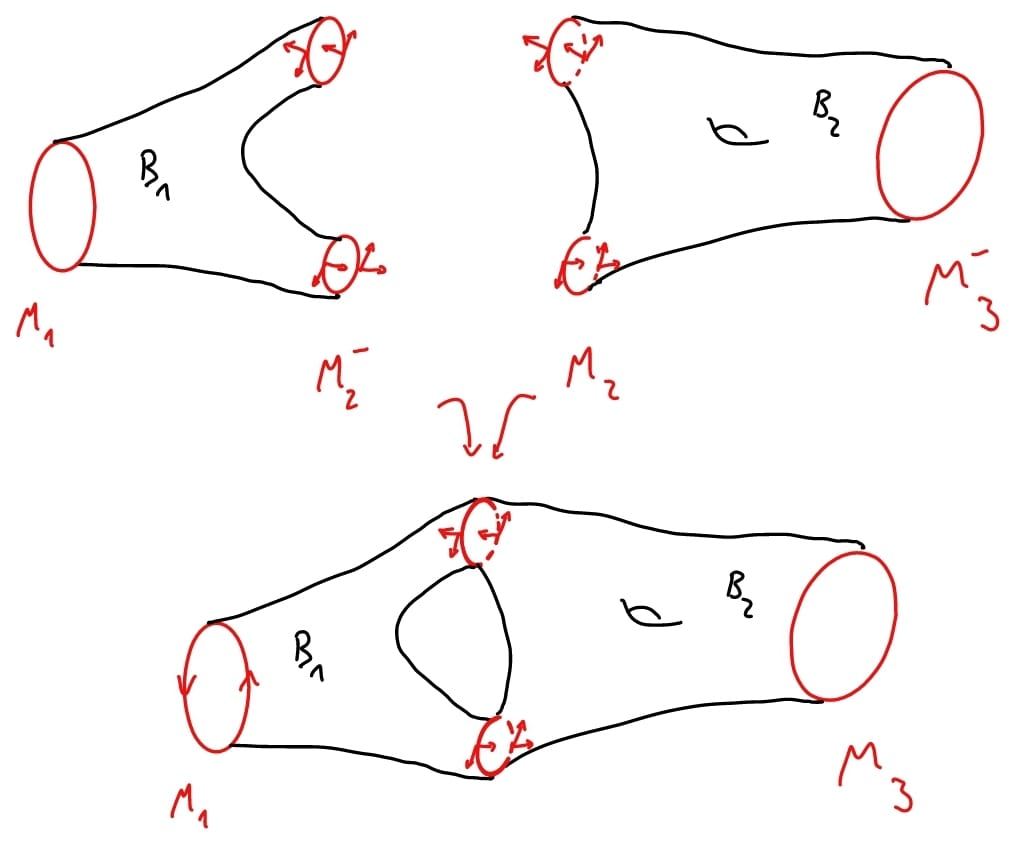
\includegraphics[width=0.6\textwidth]{ortransitivity.jpg}
        \end{center}
        %Again, here the reversed orientation is important. We have flipped the orientation of both \(N\) now once, giving them the same orientation now and can glue them together without any problems on orientations.
    \end{itemize}
\end{proof}
%This should probably be done in more detail.

\begin{definition}[oriented bordism group {\cite[p.202, 2]{atiyah}}]
    The equivalence classes of the oriented bordism relation called \demph{oriented bordism classes} and the set of oriented bordism classes of \(n\)-dimensional singular oriented manifolds in \(X\) is denoted by \(\Omega_n(X)\). \(\Omega_n(X)\) is called the \(n\)\demph{-th oriented bordism group} of \(X\)
    \[\Omega_n(X)=\{\text{closed singular oriented \(n\)-manifolds in } X\}\big/\text{oriented bordism}\]
\end{definition}

Up until now, everything seems to work out the same as in the unoriented case, but we will now see a critical difference.

\begin{observation}
    As in the oriented case, any odd number of points is not nullbordant, but now, an even number does not guarantee \(\coprod_i\{\pt\}\) being nullbordant. For instance, \((\pt,+)\) and \((\pt,-)\) are not bordant.
\end{observation}

\begin{theorem}
    The oriented bordism groups are abelian groups via the operation \(+\)
\end{theorem}

\begin{proof}
    See proof of theorem\ \ref{group structure}. The only thing that changes is the inverse element. Note that the elements are not self-inverse anymore, as \((M,f)\) and \((M,f)\) being bordant only gives us that \((M,f)+(M^-,f)\) is nullbordant, and in general, \(M\todo{\neq} M^-\). So the inverse for \([M,f]\) exists, but is \([M^-,f]\) rather than \([M,f]\).
    %For this proof, the only thing we need to change is for the existence of the inverse. We have seen in an example (to be added) that the elements are not self-inverse anymore. The inverse of \([M,f]\) is now given by \([-M,f]\). We have seen in the proof of\ \ref{oriented eq. rel} that \([M,f]+[-M,f]=0\).
\end{proof}

So, \(\Omega_n(X)\) is not a \(\mathbb{F}_2\)-vector space anymore! This makes \(\Omega_n(X)\) harder to compute.

The graded ring \(\Omega_\ast\) and the graded module \(\Omega_\ast(X)\) are defined in the same way as in the unoriented case (definitions\ \ref{bordism ring},\ \ref{bordism module}).

%I still need to see that this is ok with the orientation.

\subsubsection{Relative Oriented Bordism}

The path from absolute oriented bordism to relative oriented bordism is exactly the same as in the unoriented case. We just always need to remember that we reverse the orientations for the second singular oriented manifold. Relative oriented bordism extends the equivalence relation to not necessarily closed singular oriented manifolds.

Again, \(\Omega_n(X,A)\) is not a \(\mathbb{F}_2\)-vector space. So we get a more complicated homology theory now.

\subsubsection{Oriented Bordism Homology}

\begin{lemma}
    Relative oriented bordism is a covariant functor
    \[\Omega_\ast:\mathrm{TOP}^2\to\text{graded }\Omega_\ast\text{ modules}\]
\end{lemma}

\begin{proof}
    See proof of lemma\ \ref{functoriality}.
\end{proof}

\begin{lemma}[Naturality of the boundary map]
    The following diagram commutes for \(f:(X,A)\to(Y,A)\), \(n\in\Z\):
    \begin{center}
        \begin{tikzcd}
            {\Omega_n(X,A)} \arrow[r, "\partial_n"] \arrow[d, "f_\ast"'] & {\Omega_{n-1}(A)}  \arrow[d, "{\left(f\restrict{A}\right)}_\ast"] \\
            {\Omega_n(Y,B)} \arrow[r, "\partial_n"]  & {\Omega_{n-1}(B)}
        \end{tikzcd}
    \end{center}
\end{lemma}

\begin{proof}
    See proof of lemma\ \ref{naturality}
\end{proof}

\begin{lemma}[Homotopy invariance\ {\cite[Lemma \(2\cdot1\)]{atiyah}}]
    Let \(f,g:(X,A)\to(Y,B)\) be homotopic maps. Then \(f_\ast,g_\ast:\Omega_n(X,A)\to\Omega_n(Y,B)\) are the same homomorphisms.
\end{lemma}

\begin{proof}\cite{atiyah},\ \cite{conner}
    %Let \(h:(X,A)\times I\to (Y,B)\) be a homotopy between \(f_0\) and \(f_1\).\\
    The proof is exactly the same as the proof of lemma\ \ref{htpy inv}; noting that the cylinder is now oriented and \(\partial M\times I\) is now \(\partial I\times (M\cup M^-)=M\dis M^-\)%\((\partial I\times M)\cup (I\times M^-)\).
\end{proof}
%Maybe do this more precisely.

\begin{lemma}[Long exact sequence,\ \cite{conner}]
    The sequence
    \[\cdots\xrightarrow{\partial}\Omega_n(A)\xrightarrow{i_\ast}\Omega_n(X)\xrightarrow{j_\ast}\Omega_n(X,A)\xrightarrow{\partial}\Omega_{n-1}(A)\xrightarrow{i_\ast}\cdots\]
    is exact.
\end{lemma}

\begin{proof}\cite{conner}
    The proof is exactly the same as in the unoriented case, up to one minor adjustment. For exactness at \(\Omega_n(X,A)\), we identify the boundaries of \((M,f)\) and \((B^-,F)\); \(B\) with the opposite orientation.
\begin{comment}
    \begin{itemize}
        \item \textbf{Exactness at \(\Omega_n(A)\)}: \(i_\ast\circ\partial=0\), as \((M,f)\) is a nullbordism for \(i_\ast\circ\partial(M,f)=\partial(M,f)\)\\
        For a nullbordism \((B,g)\) of \(M,f\), \(\partial(B,g)=(M,f)\).
        \item \textbf{Exactness at \(\Omega_n(X)\)}: 
        \(j_\ast\circ i_\ast=0\) exactly as in the unoriented case.

        \item \textbf{Exactness at \(\Omega_n(X,A)\)}: 
    \end{itemize}
\end{comment}
\end{proof}

\begin{remark}
    We used lemma\ \ref{almost excision} in the proof. The oriented version of this lemma also holds, by the same proof, just keep in mind that \(M\times\{1\}\) and \(N\times\{1\}\) have negative orientation.
\end{remark}

\begin{lemma}[Excision axiom,\ {\cite[5.7]{conner}}]
    If \(\overline{U}\subset\overset{\circ}{A}\), then \(i:(X\setminus U, A\setminus U)\subset (X,A)\) induces an isomorphism of relative oriented bordism groups:
    \[i_\ast:\Omega_n(X\setminus U,A\setminus U)\xrightarrow{\cong}\Omega_n(X,A)\]
\end{lemma}

\begin{proof}\cite{conner}
    Again, everything stays the same as the proof of lemma \ref{excision}. The used lemmas\ \ref{plemma} and\ \ref{plemma2} are left unbothered by the orientations.
\end{proof}

\begin{lemma}[Disjoint union axiom]
    Relative oriented bordism satisfies the disjoint union axiom.
\end{lemma}

\begin{proof}
    See proof of lemma\ \ref{disjoint union}
\end{proof}

%\begin{observation}
%    Relative oriented bordism does not satisfy the dimension axiom.
%\end{observation}

\begin{remark}
    The dimension axiom does not hold. Seeing this is harder than in the unoriented case, but for dimension 4 the signature map gives an isomorphism
    \[\mathrm{sign}:\Omega_4\xrightarrow{\cong}\Z\]
    This map is well-defined, because the signature is a bordism invariant in every dimension, but we will not show this here.
\end{remark}

We conclude:
\begin{theorem}
    Relative oriented bordism is an extraordinary homology theory satisfying the disjoint union axiom.
\end{theorem}

\subsubsection{Calculations}

Let us try to calculate \(\Omega_n\) for low \(n\).\\
\todo{For \(n=0\), we need to see if a disjoint union of oriented points is nullbordant. 
An orientation of such spaces is a choice of a sign for every point. 
We know that \((\pt,+)\) and \((\pt,-)\) are bordant by the interval, and that \((\pt,+)\) is not bordant to itself, again by classifying compact \(1\)-manifolds, as in the unoriented case. 
So, we get an isomorphism \(\Omega_0\cong\Z\) by \[\coprod_{i=0}^n(\pt,+)\dis\coprod_{i=0}^k(\pt,-)\mapsto n-k.\]}
For \(n=1\), we see \(\Omega_1\cong\{0\}\) by seeing that \(S^1\) with any orientation has \(D^2\) with corresponding orientation as nullbordism. \(S^1\) is the only connected closed 1-manifold.\\
For \(n=2\), our problem from the unoriented case has been solved, as singular manifolds are oriented now and any connected sum of \(\mathbb{RP}^2\)s is not orientable. 
So, by the argumentation of the unoriented case, we get \(\Omega_2\cong\{0\}\).\\
Again, from dimension 3 onwards, calculations are difficult, so we will just state the results of\ \cite[\S 17]{stasheff}: We only have \(\Omega_n\cong 0\) for \(n\in\{1,2,3,5,6\}\) (and, of course, negative \(n\)). Else, we have:
\[\Omega_n\cong\begin{cases}\Z & n=0\\
\Z & n=4\\
\F_2 & n=5\\
\Z\oplus\Z & n=8\\
\F_2\oplus\F_2 & n=9\\
\dots
\end{cases}\]
Just like in the unoriented case, the oriented bordism groups have been completely determined.

We can define the \demph{reduced oriented bordism homology} analogously to reduced unoriented bordism homology.
\[\tilde\Omega_n(X):=\ker(\Omega_n(X)\to\Omega_n)\]
By the same arguments as in the unoriented case, we get 
\[\Omega_n(S^k)\cong\Omega_n\oplus\Omega_{n-k}\]


\section{Cobordism}
Now that we have seen that bordism is a homology theory, we can ask the question wether there is a dual to this, giving rise to a cohomology theory. The answer is yes, as we will see now.\\
%I should give a explanation of how \(O(n)\) (real bundles) and \(SO(n)\) (oriented real bundles) come into play.

\subsection{Cobordism}

\subsubsection{(Thom) Spectra}

\begin{definition}[Local trivialization\ {\cite[p.242]{tu}}]
    Let \(E,B,F\) be manifolds. A \demph{local trivialization} for a smooth surjective map \(\pi:E\to B\) is a collection of charts \(\{(U_i,\varphi_i)\}_{i\in I}\) (for \(\{U_i\}\) an open cover of \(M\)) such that \(\pi^{-1}(U_i)\) is diffeomorphic to \(U_i\times F\) via \(\varphi_i\) for all \(i\in I\). The charts are called \demph{trivializing charts}.
\end{definition}

\todo{Unsure if I need this.}

%\begin{definition}[Fibre bundle\ {\cite[p.242]{tu}}]
%    Let \(E,B,F\) be manifolds. A \demph{fibre bundle} is a smooth surjective map \(\pi:E\to B\) with a local trivialization with fibre \(F\).
%    \(E\) is called the \demph{total space}, \(B\) the \demph{base space} and \(F\) the \demph{fibre} of the fibre bundle.
%\end{definition}

%Maybe I will not need this Probably

\begin{definition}[Principal bundle {\cite[\nopp I.11]{tomdieck}}]
    Let \(G\) be a topological group, \(r:E\times G\to E\), \(r(x,g)=xg\) be a free right action on \(E\), and \(p:E\to B\) a continuous map. Then \((p,r)\) is called a \(G\)\demph{-principal bundle}, if 
    \begin{itemize}
        \item \(\forall g\in G, x\in E: p(xg)=p(x)\)
        \item \(\forall b\in B\exists\) a neighbourhood \(U\) and a \(G\)-homeomorphism \(\varphi:p^{-1}(U)\to U\times G\) which is a local trivialization of \(p\) over \(U\). \(\varphi\) is given by \(((u,x),g)\mapsto (u,xg)\).
    \end{itemize}
\end{definition}

\begin{definition}[Numerable cover]
    Let \(X\) be a topological space, and \(\{U_i \}_{i\in I}\) an open cover of \(X\). \(\{U_i\_{i\in I}\}\) is called \demph{numerable} if it admits a partition of unity subordinate to this cover.
\end{definition}

\begin{remark}
    For \(X\) a manifold, every cover is numerable, as manifolds are paracompact.
\end{remark}

\begin{definition}[Numerable bundle {\cite[\nopp IX.4]{tomdieck}}]
    A vector bundle \(\xi:E\to B\) is called \demph{numerable} if there exists a numerable cover \(\{U_i \}_{i\in I}\) of \(B\) such that \(\xi\) is trivial over each \(U_i\).
\end{definition}

\begin{definition}[Universal bundle {\cite[\nopp IX.4]{tomdieck}}]
    A \(G\)-principal bundle \(\xi:EG\to BG\) is called \demph{universal}, if it is numerable and for every numerable \(G\)-principal bundle \(\eta:E\to B\) has a unique bundle map to \(\xi\) (up to homotopy).
\end{definition}

\begin{remark}
    The universal \(G\)-bundle exists for every topological group \(G\) and is unique up to homotopy equivalence, in particular, \(EG\) and \(BG\) are unique up to homotopy equivalence.
\end{remark}

\begin{definition}[Classifying space {\cite[\nopp IX.4]{tomdieck}}]
    Let \(G\) be a topological group. The \demph{classifying space} \(BG\) of \(G\) is the base space of the universal principal \(G\)-bundle.
\end{definition}

\begin{observation}
    \[BO(n)=\mathbb{G}_{k,\infty}\]
    \[BSO(n)=\widetilde{\mathbb{G}}_{k,\infty}\]
\end{observation}

\todo{I might adjust this to be more like\ \cite{thom}'s definition.}
\begin{definition}[Thom space\cite{brocker}, {\cite[p.29]{thom}}, {\cite[p.201]{atiyah}}]
    Let \(\xi:E\to B\) be a real \(k\)-dimensional vector bundle over a compact manifold \(B\).
    Then the Thom space of \(\xi\) is defined as\[M(\xi)=E^c\] the one-point compactification of the total space of \(\xi\), the added point serving as the base point.\\
    Alternatively (without compact assumption):\\
    Let \(\xi:E\to B\) be a real vector bundle with Riemannian metric over a manifold \(B\). Its \demph{disk bundle} is defined by \(D(\xi):DE\to X\), \(DE=\{v\in E\mid \lVert v\rVert \leq 1\}\) and similarly, the \demph{sphere bundle} is defined by \(S(\xi):SE\to X\), \(SE=\{v\in E\mid \lVert v\rVert = 1\}\). Then the Thom space of \(\xi\) is defined as
    \[M(\xi)=D(\xi)\big/S(\xi)\]
    where the sphere bundle is collapsed to a point. We can also get the Thom space without a choice of a Riemannian metric, but I will omit this here.\\
    For \(\xi\) the universal principal \(G\)-bundle, we can write \(M(G)\) instead of \(M(\xi)\).
\end{definition}

\begin{definition}[\(MO(n), MSO(n)\)\ \cite{brocker}]
    \[MO(n):=M(\xi_{n,\infty})\] with \(\xi_{n,\infty}\) being the universal real vector bundle over \(\mathbb{G}_{k,\infty}\).
    \[MSO(n):=  \]
\end{definition}
Maybe it is enough to just say that these are called this way because the Grassmannians are the classifying spaces of \(O(n), SO(n)\) instead of defining classifying spaces.

\begin{definition}[Spectrum\ {\cite[Definition IV.1.1.]{brocker}}]
    A \demph{spectrum} \(\underline E = \{(E_n,\sigma_n)\mid n\in\mathbb{Z}\}\) is a sequence of pointed spaces \(E_n\) with pointed \demph{structure maps}\[\sigma_n:\sus E_n\to E_{n+1}\]
    where \(\sus\) denotes the reduced suspension functor.
\end{definition}

\begin{example}[Sphere spectrum]
    
\end{example}

\begin{example}[Thom spectrum\ {\cite[Beispiel IV.1.2(b)]{brocker}}]
    Let \(\gamma_{n,\infty}\) be the universal real vector bundle over \(BO(n)=\mathbb{G}_{n,\infty}\)
\end{example}

\begin{definition}[Suspension sequence]\label{suspension}
    Let \(X, Y\) be pointed spaces. We denote by \({[X,Y]}\) the set of homotopy classes of pointed maps \(X\to Y\). Then we have the \demph{suspension sequence}:
    \[[X,Y]\to[\sus{X},\sus{Y}]\to\dots\to[\sus^n{X},\sus^n{Y}]\] 
\end{definition}


\begin{theorem}[\todo{Freudenthal suspension theorem}]\label{freudenthal}
    Let \((X,Y)\) be a pair of spaces. Then for large enough \(n\), the suspension map
    \[[\sus^n X,\sus^n Y]\to[\sus^{n+1}X,\sus^{n+1}Y]\]
    is an isomorphism.
\end{theorem}

\begin{proof}
    omitted.
\end{proof}

%\begin{lemma}\label{natural map}\cite{thom}
%    The natural map
%    \[\sus\{MSO(n)\}\to MSO(n+1)\]
%    induces isomorphisms of homotopy groups \(\pi_{n+1}\) for \(n\) large.
%\end{lemma}

%\begin{corollary}[{\cite[p.201]{atiyah}}]
%    For a finite CW-complex \(X\) with basepoint, \[[X,\sus\{MSO(n)\}]\to[X,MSO(n+1)]\] is bijective for \(n\) large.
%\end{corollary}

%\begin{lemma}[{\cite[p.201]{atiyah}}]
%    Let \(Y\) be a subcomplex of a CW-complex \(X\). Then from\ \ref{suspension} and\ \ref{natural map}, we get a map
%    \[[\sus^{n-k}(X\big/ Y),MSO(n)]\to[\sus^{n+1-k}(X\big/Y, MSO(n+1))]\]
%\end{lemma}

%\begin{definition}[Reduced cohomology associated to a spectrum]
    
%\end{definition}

\begin{theorem}[Cohomology theory associated to a spectrum]\label{spectrum cohomology}
    Let \(\underline{E}\) be a spectrum. Then the following is a cohomology theory.
    \[\h^k(X,Y;\underline{E}):=\lim_{n\to\infty}[\sus^{n-k}(X\big/Y),E_n]\]
\end{theorem}

\begin{definition}[Cobordism group\ {\cite[p.201]{atiyah}}]
    Let \((X,Y)\) be a pair of spaces, then for \(k\in\mathbb{Z}\), the \(k\)\demph{-th oriented cobordism group} is
    \[\Omega^k(X,Y):=\h^k(X,Y;MSO)=\lim_{n\to\infty}[\sus^{n-k}(X\big/Y),MSO(n)]\]
    with respect to the above map.
    Analogously, we define the \demph{relative unoriented cobordism group} as
    \[\mathfrak{N}^k(X,Y):= \h^k(X\big/Y;MO)=\lim_{n\to\infty}[\sus^{n-k}(X\big/ Y),MO(n)]\]
\end{definition}

So, proving theorem\ \ref{spectrum cohomology} gives us that cobordism defines a cohomology theory. Again, we need to check axioms.\\
Proving theorem\ \ref{spectrum cohomology} will be the goal of\ \ref{cohomology}

\subsubsection{\todo{The Eilenberg-Steenrod Axioms}}
To get a the axioms for cohomology theories, intuitively, we \enquote{reverse all arrows} in the previously defined axioms for homology theories in\ \ref{es axioms}.

\begin{definition}[Cohomology theory\ {\cite[Definition 5.2]{luck}}]
    A \demph{cohomology theory} \(\mathcal{H}^\ast=(\mathcal{H}^\ast,\partial^\ast)\) with coefficients in \(R\)-modules is a contravariant functor \[\mathcal{H}^\ast:\mathrm{TOP}^2\to\mathbb{Z}\text{-graded }R\text{-modules}\] together with a natural transformation \[\partial^\ast:\mathcal{H}^\ast\circ I\to\mathcal{H}^{\ast+1}\] satisfying the following axioms:
    \begin{itemize}
        \item \textbf{Homotopy invariance} For homotopic maps of pairs \(f,g:(X,A\to Y,B)\), we have \[\mathcal{H}^n(f)=\mathcal{H}^n(g):\mathcal{H}^n(Y,B)\to\mathcal{H}^n(X,A)\]
        \item \textbf{Long exact sequence} For a pair of spaces \((X,A)\), the sequence \[\dots\xrightarrow{\partial^{n-1}}\mathcal{H}^n(X,A)\xrightarrow{\mathcal{H}^n(j)}\mathcal{H}^n(X)\xrightarrow{\mathcal{H}^n(i)}\mathcal{H}^n(A)\xrightarrow{\partial^n(X,A)}\mathcal{H}^{n+1}(X,A)\rightarrow\dots\] is exact, where \(i:A\hookrightarrow X\) and \(j:(X,\emptyset)\hookrightarrow (X,A)\) are the inclusions.
        \item \textbf{Excision} Let \((X,B,A)\) be a triple of spaces such that \(\overline{A}\subseteq\overset{\circ}{B}\). Then the inclusion map \(i:(X\setminus A,B\setminus A)\hookrightarrow(X,B)\) induces an isomorphism of cohomology groups: \[\mathcal{H}^n(i):\mathcal{H}^n(X,B)\xrightarrow{\cong}\mathcal{H}^n(X\setminus A, B\setminus A)\]
    \end{itemize}
    Sometimes one adds the following axioms:
    \begin{itemize}
        \item \textbf{Disjoint union axiom}
        For a disjoint union of spaces \(\coprod_{i\in I}X_i\) over any index set \(I\) and the inclusions \(j_i:X_i\to\coprod_{i\in I}X_i\), the map
        \[\prod_{i\in I}\mathcal{H}^n(j_i):\mathcal{H}^n\left(\coprod_{i\in I X_i}\right)\xrightarrow{\cong}\prod_{i\in I}\mathcal{H}^n(X_i)\]
        \item \textbf{Dimension axiom}
        For all \(n\in\mathbb{Z}\), we have \[\mathcal{H}^n(\{\mathrm{pt}\})\cong\begin{cases} R, & n=0\\ 0, & n\neq0\end{cases}\]
    \end{itemize}
\end{definition}

\subsubsection{Bordism Cohomology}\label{cohomology}
To prove theorem\ \ref{spectrum cohomology}, we will check the axioms one by one. For this section, we will fix a spectrum \(\underline{E}\), and \(\h^\ast\) will be the associated map, as defined in theorem\ \ref{spectrum cohomology}.

\begin{lemma}[Functoriality]\label{cofunctoriality}
    \(\h^\ast\) defines a contravariant functor
    \[\h^\ast:\mathrm{TOP}^2\to \text{graded abelian groups}\]
\end{lemma}

\begin{remark}
    Every abelian group is a \(\Z\)-module.
\end{remark}

\begin{proof}
    Let \((X,A)\in\mathrm{Ob}(\mathrm{TOP}^2)\). Then \(\h^\ast(X,A)=\lim_{n\to\infty}[\sus^{n-k}(X\big/A),E_n]\) is an abelian group, as for every \(n,k\), \([\sus^{n-k}(X\big/A),E_n]\) is an abelian group and the limit of a sequence of abelian groups is an abelian group.\\
    Now, for a map \(f\in\mathrm{Mor}(\mathrm{TOP}^2)\), \(f:(X,A)\to(Y,B)\), we get a map
    \[f_\ast:=\h^\ast(f):\lim_{n\to\infty}[\sus^{n-k}(Y\big/B),E_n]\to\lim_{n\to\infty}[\sus^{n-k}(X\big/A,E_n)]\]
    by
    \[x\mapsto x\circ \lim_{n\to\infty}f_n\]
    where \[f_n:\sus^{n-k}(X\big/A)\to\sus^{n-k}(Y\big/A)\]
    is the map such that the following diagram commutes:
    \begin{center}
        \begin{tikzcd}
            {(X,A)} \arrow[r, "f"] \arrow[d, "\sus^{n-k}\circ q"'] & {(Y,B)}  \arrow[d, "\sus^{n-k}\circ q"] \\
            {\sus^{n-k}(X\big/A)} \arrow[r, "f_n"]  & {\sus^{n-k}(Y\big/B)}
        \end{tikzcd}
    \end{center}
    where \(q:(X,A)\to X\big/A\) is the quotient map.\\
    Then we have that \(\h^\ast(\id_{(X,A)})=\id_{\h^\ast(X,A)}\), as all \(f_n=\id\) for every \(n\).\\
    For \(f:(X,A)\to(Y,B)\), \(g:(Y,B)\to(Z,C)\), we have, for \(x\in\h^\ast(Z,C)\)
    \[(g\circ f)^\ast(x)=x\circ\lim_{n\to\infty}(g\circ f)_n=x\circ\lim_{n\to\infty}(g_n\circ f_n)\]\[=x\circ\lim_{n\to\infty}g_n\circ\lim_{n\to\infty}f_n=g^\ast(x)\circ\lim_{n\to\infty}f_n=f^\ast(g^\ast(x))\]
    %Thus, \((g\circ f)^\ast=f^\ast\circ g^\ast\), so \(\h^\ast\) is contravariant.
\end{proof}

\begin{lemma}[Naturality]
    The boundary operator
    \[\partial^\ast:\h^{\ast-1}(A)\to\h^\ast(X,A)\]
    is given by \todo{?the suspension homomorphism?}
\end{lemma}

\begin{observation}
    The homotopy invariance axiom is satisfied by the defintion of the cohomology groups as set of homotopy classes of maps.
\end{observation}

\begin{lemma}[Long exact sequence]
    
\end{lemma}

\begin{lemma}[Excision]
\end{lemma}

\begin{lemma}[Disjoint union axiom]
\end{lemma}

\begin{observation}[Dimension axiom]
\end{observation}


\begin{proof}[Proof of theorem\ \ref{spectrum cohomology}]
    
\end{proof}

Conclude:
\begin{theorem}[Bordism cohomology theory]
\end{theorem}

\subsection{Duality to Bordism Homology}

%\subsubsection{Calculations}

%\todo{I could cite the original axioms of Eilenberg-Steenrod\ \ref{eilenberg}}

%Thom isomorphism, Thom class, Thom isomorphism theorem

%\section{Pontryagin-Thom Construction}

\newpage
\addcontentsline{toc}{section}{References}
\printbibliography%
\end{document}